\documentclass[a4paper]{article}

%Moduli utilizzati
\usepackage[italian]{babel}
\usepackage[utf8]{inputenc}
\usepackage{titling}
\usepackage{graphicx}
\usepackage{float}
\usepackage[nottoc]{tocbibind}
\usepackage{tabularx}
\usepackage{longtable}
\usepackage{hyperref}  
\usepackage{xspace}
\usepackage{listings}
\lstloadlanguages{SQL} 
\usepackage{tikz}
\usepackage{colortbl}
\usepackage[titletoc]{appendix}

%Setup
\hypersetup{
    colorlinks,
    citecolor=black,
    filecolor=black,
    linkcolor=black,
    urlcolor=black
}

\lstset{
  columns = fullflexible,
  keywordstyle = \color{black}\bfseries, 					
  commentstyle = \color{blue},
  language = SQL,  
  linewidth = 1 \textwidth, 
  frame = tb, 
  breaklines = true, 
  extendedchars = true
}

%Nuovi comandi
\newcommand{\subtitle}[1]{%
  \posttitle{%
    \par\end{center}
    \begin{center}\large#1\end{center}
    \vskip0.5em}%
}

\newcommand{\net}{Ne-t\xspace}
\newcommand{\mytitle}{PadovaCard}
\newcommand{\mydegree}{Tesi di Laurea Triennale}
\newcommand{\glossario}[1]{\textit{#1\ped{\ped{G}}}}
%\newcommand{\glossario}[1]{#1}
\newcommand{\definizione}[1] {\textbf{#1}:}
\newcommand{\vivaticket}{VivaTicket\xspace}
\newcommand{\tlite}{Tlite\xspace}
\newcommand{\charta}{Charta\xspace}
\newcommand{\cappella}{Cappella degli Scrovegni\xspace}


\pagestyle{myheadings}
\markright{Nicolò Tresoldi - PadovaCard}

\title{PadovaCard}
\subtitle{Attività di stage esterno}
\author{Nicolò Tresoldi}


%Inizio Documento
\begin{document}

%\begin{titlepage}

\begin{center}

\begin{LARGE}
\textbf{Università degli Studi di Padova}\\
\end{LARGE}

\vspace{10pt}

\begin{Large}
\textsc{Dipartimento di Matematica}\\
\end{Large}

\vspace{10pt}

\begin{large}
\textsc{Corso di laurea in Informatica}\\
\end{large}

\vspace{30pt}
\begin{figure}[htbp]
\begin{center}

\includegraphics[height=6cm]{images/logo-unipd.png}
\end{center}
\end{figure}
\vspace{30pt} 

\begin{LARGE}
\begin{center}
\textbf{\mytitle}\\
\end{center}
\end{LARGE}

\vspace{10pt} 

\begin{large}
\textsl{\mydegree}\\
\end{large}

\vspace{40pt} 

\begin{large}
\begin{flushleft}
\textit{Relatore}\\ 
\vspace{5pt} 
Prof. Mauro Conti
\end{flushleft}

\vspace{0pt} 

\begin{flushright}
\textit{Laureando}\\ 
\vspace{5pt} 
Nicolò Tresoldi
\end{flushright}
\end{large}

\vspace{40pt}

\line(1, 0){338} \\
\begin{normalsize}
\textsc{Anno Accademico 2014/2015}
\end{normalsize}

\end{center}
\end{titlepage} 
%% !TEX encoding = UTF-8
% !TEX TS-program = pdflatex
% !TEX root = ../tesi.tex
% !TEX spellcheck = it-IT

%**************************************************************
% Colophon
%**************************************************************
\clearpage
\phantomsection
\thispagestyle{empty}

\hfill

\vfill

\noindent Nicolò Tresoldi: \textit{\mytitle,}
\mydegree,
\textcopyright\ Marzo 2015.
\maketitle

\tableofcontents

\listoftables

\listoffigures

%\newpage

%Capitoli

%\section{Introduzione}

\subsection{PadovaCard ora}
PadovaCard è un pacchetto ideato per chi desidera visitare la città. 
I punti di forza sono:
\begin{itemize}
\item Utilizzo gratuito dei mezzi di trasporto pubblici comunali;
\item Parcheggio gratuito in alcune zone;
\item Noleggio di veicoli, biciclette, segway a prezzo scontato;
\item Accesso gratuito alle strutture convenzionate.
\end{itemize}
\`E acquistabile con validità di 48 e 72 ore, contate dal momento in cui la PadovaCard viene ritirata allo sportello informazioni assistenza turistica (\glossario{IAT}).
La carta si presenta come in figura \ref{immaginePadovaCard}, e non presenta nessun tipo di circuito, banda magnetica o codice stampato. 
Proprio per questo motivo, nonostante sia una tessera personale e non cedibile, non c'è modo di verificare chi ne è l'intestatario.\\

\begin{figure}[H]
\centering
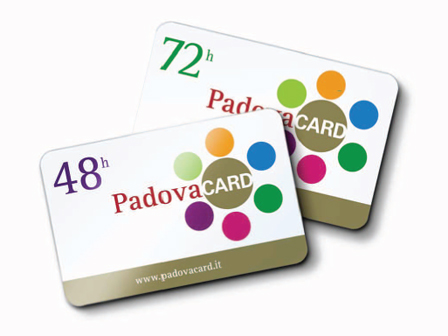
\includegraphics[width=0.6\textwidth]{images/padovacard.jpg}
\caption{Veste grafica dell'attuale PadovaCard}\label{immaginePadovaCard}
\end{figure}

Per acquistare una PadovaCard l'\glossario{utente} può recarsi ad uno degli sportelli IAT che si trovano sul territorio della città di Padova o in uno dei punti vendita autorizzati (hotel, tabaccherie, etc.).\\

\label{cappella}
La \cappella è uno tra i luoghi d'interesse più visitati, ed è convenzionato con PadovaCard. La visita alla cappella presenta un ingresso contingentato, ovvero il numero di visitatori per ogni visita è fissato, e per questo è necessario prenotare la propria visita, definendo data e fascia oraria. Non è possibile visitare la \cappella senza prenotazione. \\

Questo vincolo fa si che chiunque acquisti una PadovaCard con l'intenzione di visitare la \cappella è obbligato a prenotarne la visita. Questo è possibile farlo se si acquista la PadovaCard in un punto vendita autorizzato, oppure attraverso la piattaforma \vivaticket.
\`E inoltre attivo un call center che permette agli utenti di acquistare una PadovaCard collegata ad un ingresso in \cappella.
In questi ultimi due casi la PadovaCard verrà poi ritirata presso un punto vendita o direttamente alla \cappella.\\

I principali problemi di funzionamento dell'attuale PadovaCard sono:
\begin{itemize}
\item La PadovaCard non è nominativa;
\item Il sistema non è informatizzato e non prevede alcun tipo di tracciamento;
\item L'utente è obbligato in tutti i casi a passare da uno IAT per il ritiro della PadovaCard;
\item La piattaforma di vendita è frammentata e non comunica pienamente le offerte della PadovaCard;
\item Il sistema di vendita è frammentato tra OSS e \tlite.
\end{itemize}

La nuova PadovaCard si pone l'obbiettivo di risolvere questi problemi.



\subsection{OSS}\label{oss}
\subsubsection{Overview}
\glossario{OSS} è una piattaforma sviluppata da \net per la gestione del call center e degli sportelli \glossario{IAT} e dei relativi operatori.
Gli operatori si autenticano su questo software per gestire la vendita dell'attuale PadovaCard\footnote{Sia OSS che \tlite possono vendere la PadovaCard, salvando i dati relativi alla vendita in due diverse basi di dati. SI tratta di un problema dell'attuale sistema.} e di ogni altra merce in vendita agli sportelli \glossario{IAT}. 
OSS permette agli operatori di visualizzare il rendiconto delle vendite e al personale operatvio di compiere interrogazioni sulla base di dati.

\subsubsection{Dettagli tecnici}
Il software è scritto in \glossario{Cake Php} e si basa sull'architettura \glossario{MVC}. Come previsto da MVC sono presenti dei model, uno per ogni tabella del database, tali model si occupano di comunicare col database e di manipolare e verificare i dati che vengono estratti ed inseriti.
Per ogni model è presente un controller, che fornisce la logica al sistema attraverso vari metodi. Ad ogni controller sono collegate più view, ovvero le interfaccie utente. Una view è una pagina con cui l'utente interagisce e ogni view deve essere associata ad un controller di cui chiamerà i metodi.\\

Il database su cui si basa il sistema è un database \glossario{MySql}.

\subsection{\tlite}
\tlite è il software sviluppato da \charta che si trova dietro la piattaforma \vivaticket, e che gli operatori utilizzano per gestire la vendita delle PadovaCard\footnote{Vedi nota 1.} con annessa prenotazione alla \cappella.
Non trattandosi di un software sviluppato da \net si è dovuto adattare i requisiti ai limiti imposti da tale software.
Il limite principale è la mancanza di comunicazione tra \tlite e il software sviluppato causato da una mancanza di \glossario{API} pubbliche di \tlite.\\

Si sono comunque rivelate necessarie alcune modifiche minori al software e per questo è stato svolto un incontro tra gli sviluppaotri di \tlite e quelli di \net.
Ai fini di questo documento non è necessario conoscere il funzionamento di \tlite nel suo insieme, mentre i punti d'interesse per la progettazione del nuovo sistema per PadovaCard saranno presentati nella sezione \ref{progettazione}.

\subsection{Lavoro svolto}
Il focus dello stage è stato sui seguenti punti:
\begin{itemize}
\item Analizzare i requisiti del sistema PadovaCard, il risultato è visibile alla Sezione \ref{analisideirequisiti};
\end{itemize}

\subsubsection{Analisi dei requisiti}
Di seguito viene descritto l'approccio seguito per generare una dettagliata analisi dei requisiti, il cui risultato è presentato nella Sezione \ref{analisideirequisiti}.
L'azienda \net ha fornito al tirocinante un documento in cui vengono descritti gli obbiettivi e le criticità del nuovo sistema per la Padovacard. Dallo studio di tale documento il tirocinante ha potuto definire il piano di lavoro dello stage.\\

L'analisi degli obbiettivi e del funzionamento del sistema ad alto livello è stato poi discusso in diverse riunioni tra i membri del team di sviluppo, ponendo un focus particolare sulle difficoltà inerenti alla \cappella, esposte nella Sezione \ref{cappella}.\\

Da queste riunioni il tirocinante ha estratto i dettagli funzionali dell’applicazione.
Per esprimere in modo chiaro i requisiti individuati si è ricorso al formalismo UML - Casi d'uso, anch'essi visionabili alla Sezione \ref{analisideirequisiti}.\\

L'individuazione dei requisiti è stata fatta corretamente già alla prima iterazione, mentre i casi d'uso e la loro descrizione dettagliata sono stati modificati più volte, al fine di eliminare ogni possibile ambiguità.
\subsection{Risultati a fine stage}
%\section{Ambiente di lavoro}
\subsection{Azienda}
\subsection{Processi di sviluppo}
\subsection{Strumenti di lavoro}
%\section{Studio di fattibilità delle possibili soluzioni}
Per poter comprendere le soluzioni di seguito proposte è necessario conoscere il software \glossario{OSS}, presentato alla Sezione \ref{oss}.
La seguente immagine presenta il funzionamento del nuovo sistema PadovaCard nel suo complesso.
Per maggiori dettagli vedere l'analisi dei requisiti alla Sezione \ref{analisideirequisiti}.
\begin{figure}[H]
\centering
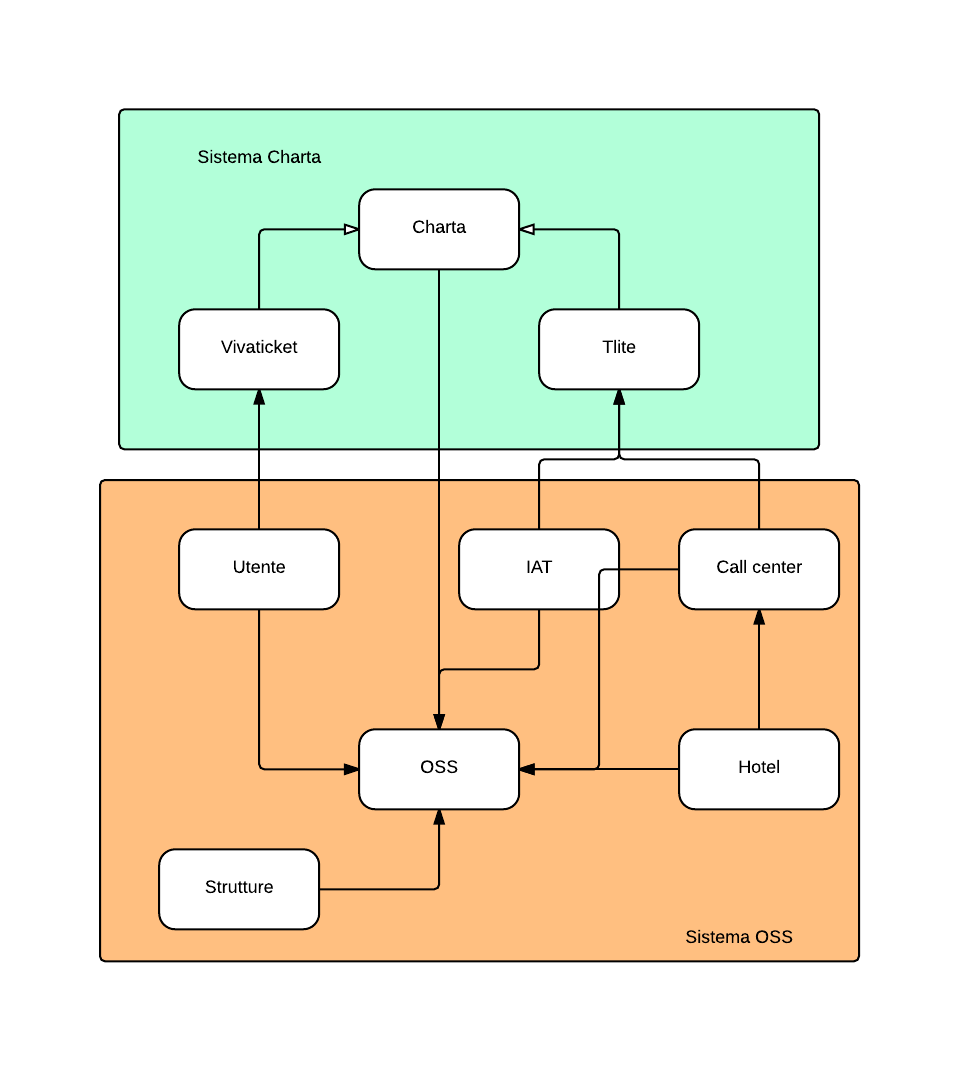
\includegraphics[width=0.9\textwidth]{images/Schema_introduttivo.png}
\caption{Architettura di alto livello di OSS}
\end{figure}

\subsection{Espansione del sistema OSS}
Per questa soluzione non è prevista la produzione di un sistema ex-novo, ma un ampliamento del sistema \glossario{OSS} già esistente affinchè soddisfi i requisiti richiesti.
\begin{figure}[H]
\centering
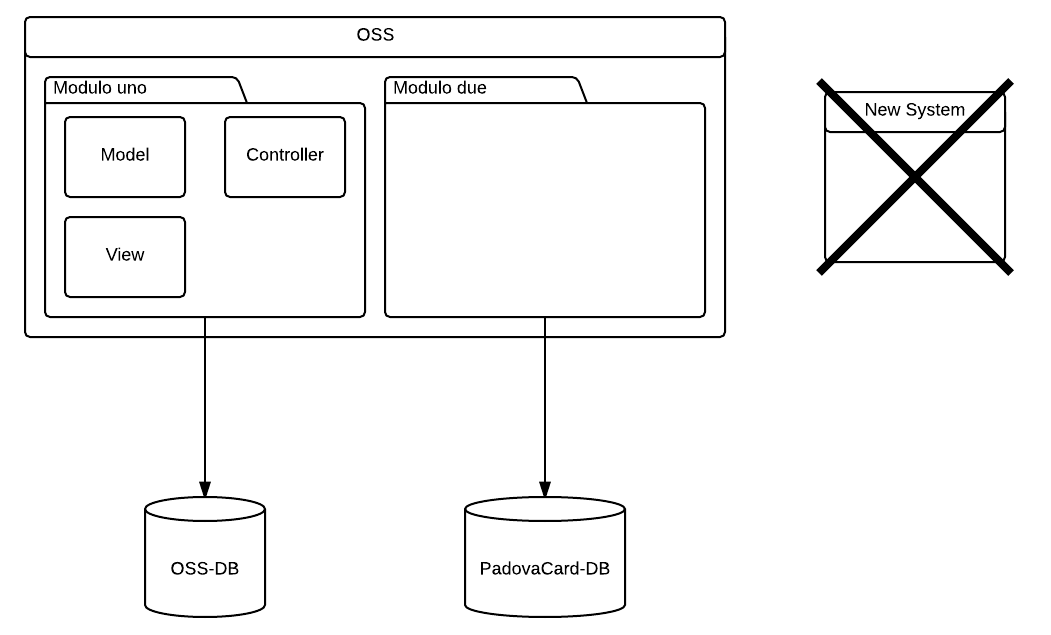
\includegraphics[width=0.7\textwidth]{images/Espansione_del_sistema_OSS.png}
\caption{Diagramma della soluzione: Espansione del sistema OSS}
\end{figure}
Nella figura tutti i componenti interni al modulo uno sono quelli già esistenti che non andranno modificati.
I componenti all'interno del modulo due sono quelli che verranno progettati e sviluppati per soddisfare i requisiti annessi alla nuova PadovaCard.\\

Il database \glossario{OSS} è quello già presente mentre il database PadovaCard è quello che andrà creato. In alternativa si può utilizzare un unico database e creare nuove tabelle per la gestione della PadovaCard.
Questa soluzione soddisfa il requisito di avere un unica piattaforma per gestire tutto, dalla vendita della PadovaCard, alla vendita di altri articoli, alla gestione dei pagamenti e degli operatori.\\

Uno svantaggio è che il tirocinante, se pur a conoscenza del linguaggio PHP e dell'architettura MVC, non ha mai sviluppato con CakePHP, inoltre dovrebbe studiare il funzionamento del sistema esistente nel dettaglio. Tale studio può limitarsi alle sezioni del software di interesse, ma si prevede un costo di apprendimento iniziale elevato.\\
\textbf{Vantaggi:}
\begin{itemize}
\item Non viene creato un nuovo sistema;
\item Necessaria meno documentazione;
\item Il pagamento di PadovaCard e altri articoli è unico;
\item I dati relativi alla PadovaCard sono logicamente separati, mentre quelli amministrativi sono accorpati.
\end{itemize}
\textbf{Svantaggi:}
\begin{itemize}
\item Necessario l'apprendimento del funzionamento di OSS;
\item Necessario l'apprendimento del funzionamento di CakePHP;
\item Rischio di introdurre errori in un sistema funzionante;
\end{itemize}

\subsection{Nuovo sistema per gli acquisti}
In questa soluzione si prevede di progettare e realizzare un nuovo sistema che si occuperà della vendita delle PadovaCard e degli altri articoli. Il sistema OSS resterà presente in parallelo per la gestione delle rimanenti necessità.

\begin{figure}[H]
\centering
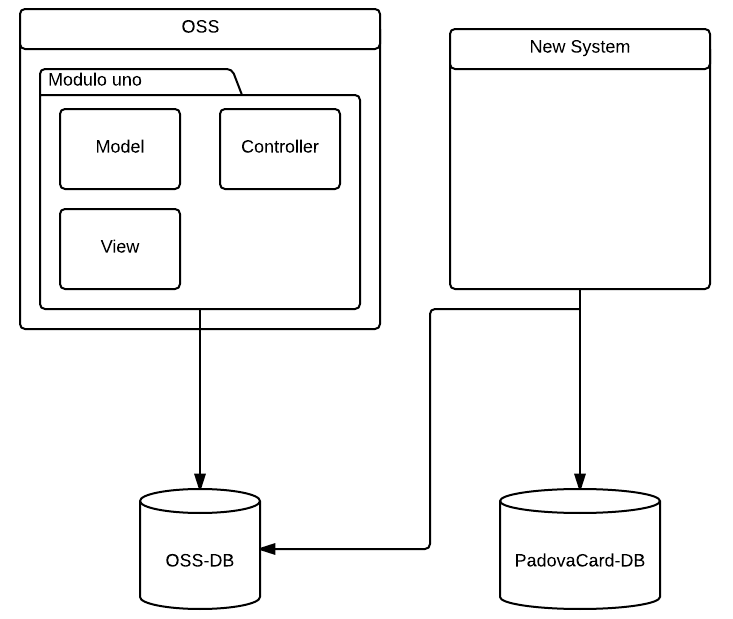
\includegraphics[width=0.7\textwidth]{images/Nuovo_sistema_per_gli_acquisti.png}
\caption{Diagramma della soluzione: Nuovo sistema per gli acquisti}
\end{figure}
A differenza della soluzione precedente in questo caso il sistema OSS ora esistente non viene modificato, e si crea un nuovo sistema, identificato in figura come come new System. Tale sistema non interagisce in alcun modo con il sistema OSS, ma comunica invece con il database OSS per la scrittura degli acquisti, mentre comunicherà con il database PadovaCard per tutti i dettagli riguardanti le sole PadovaCard.\\

Tale soluzione presenta il vantaggio per il tirocinante di non dover apprendere CakePHP e il funzionamento di OSS, ma c'è il rischio di una frammentazione dei dati. \\
\textbf{Vantaggi:}
\begin{itemize}
\item Nuovo sistema, separato ed indipendente per la vendita della PadovaCard;
\item Il sistema OSS non viene modificato;
\item Il pagamento di PadovaCard e altri articoli è unico;
\item I dati relativi alla PadovaCard sono logicamente separati, mentre quelli amministrativi sono accorpati.
\end{itemize}
\textbf{Svantaggi:}
\begin{itemize}
\item Necessaria la progettazione di un nuovo sistema;
\item Il codice sorgente relativo a vendita e pagamento verrebbe duplicato;
\item Necessaria una maggiore documentazione;
\item Si hanno due sistemi che in parte fanno la stessa cosa.
\end{itemize}

\subsection{Sistema ibrido}
Si tratta di una soluzione che ibrida le due appena viste. In questo caso viene creato un nuovo sistema, che si occuperà della sola vendita della PadovaCard (ed eventualmente dei singoli accessi ai luoghi d'interesse), mentre OSS continuerà a vendere tutti gli altri articoli. 
I due sistemi comunicheranno tra loro e l'operatore potrà passare da uno all'altro in modo automatico in base a cosa desidera vendere. \\

Il pagamento finale sarà possibile su entrambe le piattaforme e comprenderà gli articoli venduti su entrambe.

\begin{figure}[H]
\centering
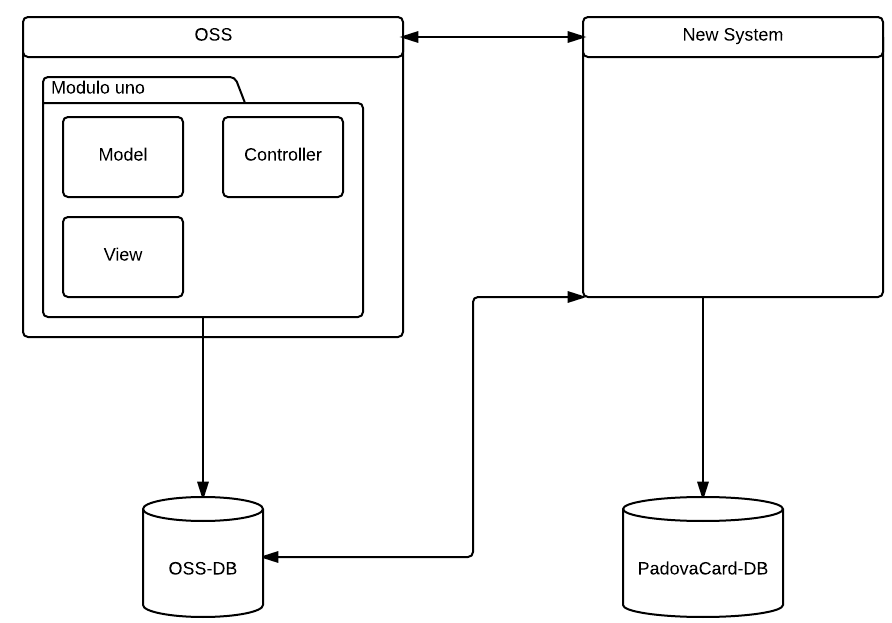
\includegraphics[width=0.7\textwidth]{images/Sistema_ibrido.png}
\caption{Diagramma della soluzione: Sistema ibrido}
\end{figure}
Questa soluzione prevede che il sistema OSS non venga modificato se non per il redirect al nuovo sistema e la conferma al nuovo sistema dell'avvenuto pagamento. 
Nel database OSS saranno salvati i record di vendita, comprese le PadovaCard, ma tutti i dettagli relativi ad esse saranno separati nel database PadovaCard (o in un'altra tabella nello stesso database). \\
\textbf{Vantaggi:}
\begin{itemize}
\item Nuovo sistema, separato ed indipendente per la vendita della PadovaCard;
\item Il sistema OSS viene modificato solo in superficie, con un costo basso;
\item Per l'operatore il pagamento di PadovaCard e altri articoli è unico;
\item I dati relativi alla PadovaCard sono logicamente separati, mentre quelli amministrativi sono accorpati.
\end{itemize}
\textbf{Svantaggi:}
\begin{itemize}
\item Necessaria la progettazione di un nuovo sistema;
\item L'operatore passando da un sistema all'altro si troverebbe una diversa interfaccia;
\item Necessaria una maggiore documentazione;
\end{itemize}

\subsection{Conclusioni}
La soluzione due, Nuovo sistema per gli acquisti, presenta maggiori svantaggi rispetto ai vantaggi, e per questo è stata immediatamente scartata. \\

Le soluzioni uno e tre hanno molti vantaggi in comune, come la separazione logica dei dati relativi alla PadovaCard e l'unificazione del sistema di pagamento, ma ritengo che la soluzione uno presenti un minor costo di sviluppo in termini di uomo/ora, e sia quindi da preferire.  
%\clearpage\null\newpage
\section{Analisi dei requisiti}\label{analisideirequisiti}
\subsection{Casi d'uso}

I casi d'uso sono presentati con la notazione \glossario{UML}.
Ad ogni caso d'uso è associato un titolo ed un codice che segue il seguente formalismo:

\begin{center}
\textbf{UC[F]\{Gerarchia\}}
\end{center}

Dove:
\begin{itemize}
\item UC sono i casi d'uso obbligatori;
\item UCF sono i casi d'uso facoltativi;
\item Gerarchia identifica la relazione gerarchica che c'è tra i requisiti di uno stesso tipo. C'è quindi una struttura gerarchica per ogni tipologia di requisito.
\end{itemize}

\subsubsection{Caso d'uso UC: Operazioni ad alto livello}\label{UC}
Il seguente diagramma presenta una visione di alto livello dei casi d'uso obbligatori. Ogni caso d'uso verrà poi analizzato nel dettaglio nelle sezioni successive. I casi d'uso opzionali si trovano dalla Sezione \ref{UCF} in poi.

\begin{figure}[H]
\centering
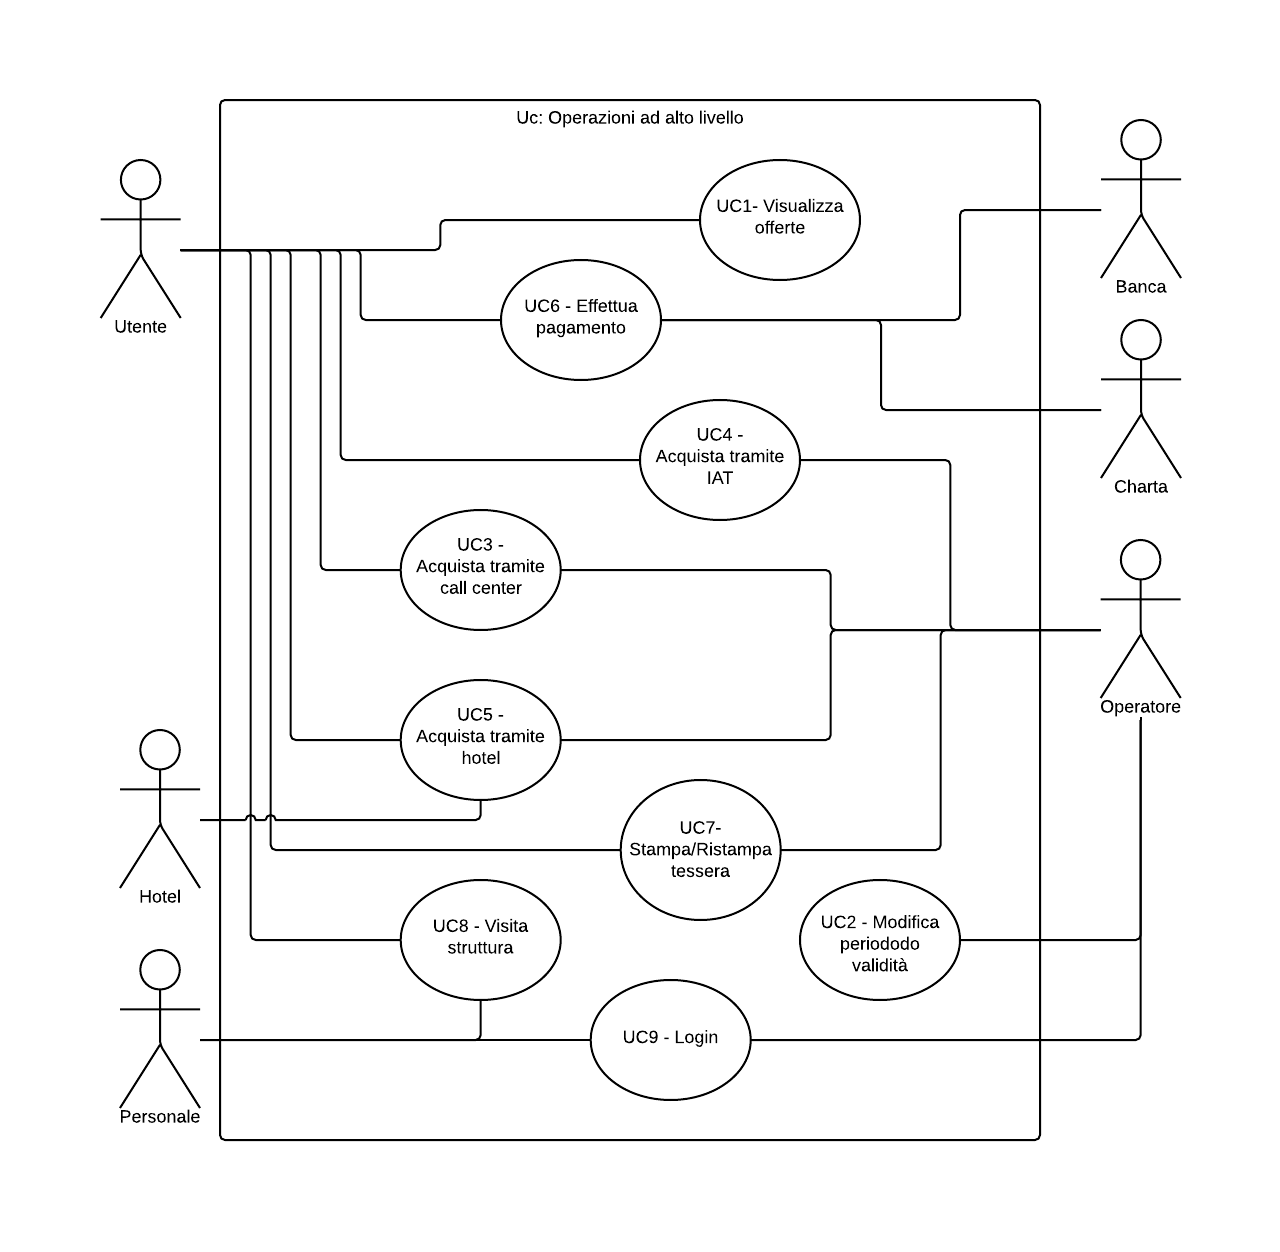
\includegraphics[width=1\textwidth]{images/UC.png}
\caption{Caso d'uso UC: Operazioni ad alto livello}
\end{figure}

\subsubsection{Caso d'uso UC1: Consultazione offerte}\label{UC1}
\begin{figure}[H]
\centering
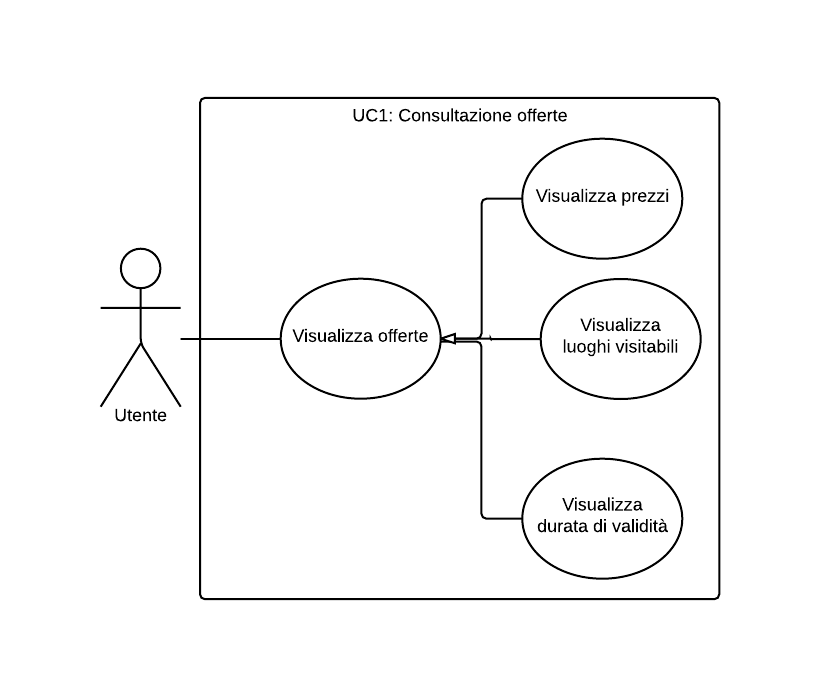
\includegraphics[width=1\textwidth]{images/UC1.png}
\caption{Caso d'uso UC1: Consultazione offerte}
\end{figure}
\begin{itemize}
\item \textbf{Attori:} Utente;
\item \textbf{Descrizione:} L'utente deve poter consultare online le offerte relative alla propria PadovaCard. Tali offerte comprendono i vari pacchetti con cui la PadovaCard viene proposta, i luoghi con essa visitabili ed i relativi costi e periodo di validità. Si tratta di un portale statico;

\item \textbf{Flusso principale degli eventi:}
	\begin{itemize}
		\item L'utente si collega al portale tramite browser;
		\item L'utente visualizza le informszioni a cui è interessato.
	\end{itemize}
\end{itemize}

\subsubsection{Caso d'uso UC2: Modifica periodo validità}
\begin{figure}[H]
\centering
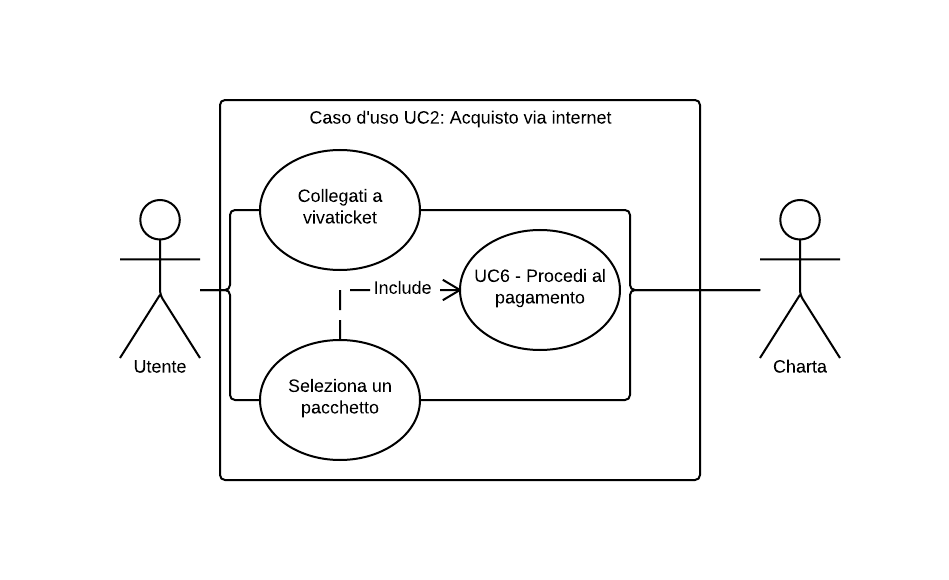
\includegraphics[width=1\textwidth]{images/UC2.png}
\caption{Caso d'uso UC2: Modifica periodo validità}
\end{figure}
\begin{itemize}
\item \textbf{Attori:} Utente, operatore;
\item \textbf{Descrizione:} L'utente ha acquistato una o più PadovaCard, e nel momento dell'acquisto ha definito il loro periodo di validità, selezionando data e ora, come descritto in UC6, alla Sezione \ref{UC6}. L'utente decide però di modificare tale periodo di validità, non gli è consentito farlo da solo, dovrà quindi contattare un operatore, call center o IAT e far modificare il peridoo di validità, con il vincolo che se è prevista una visita alla cappella degli Scrovegni, essa dovrà trovarsi sempre dentro l'arco temporale di validità della tessera;
\item \textbf{Precondizione:} L'utente desidera modificare il periodo di validità della PadovaCard;
\item \textbf{Postcondizione:}  Il periodo di validità della PadovaCard è modificato.
\end{itemize}


\subsubsection{Caso d'uso UC3: Acquisto via call center}\label{UC3}
\begin{figure}[H]
\centering
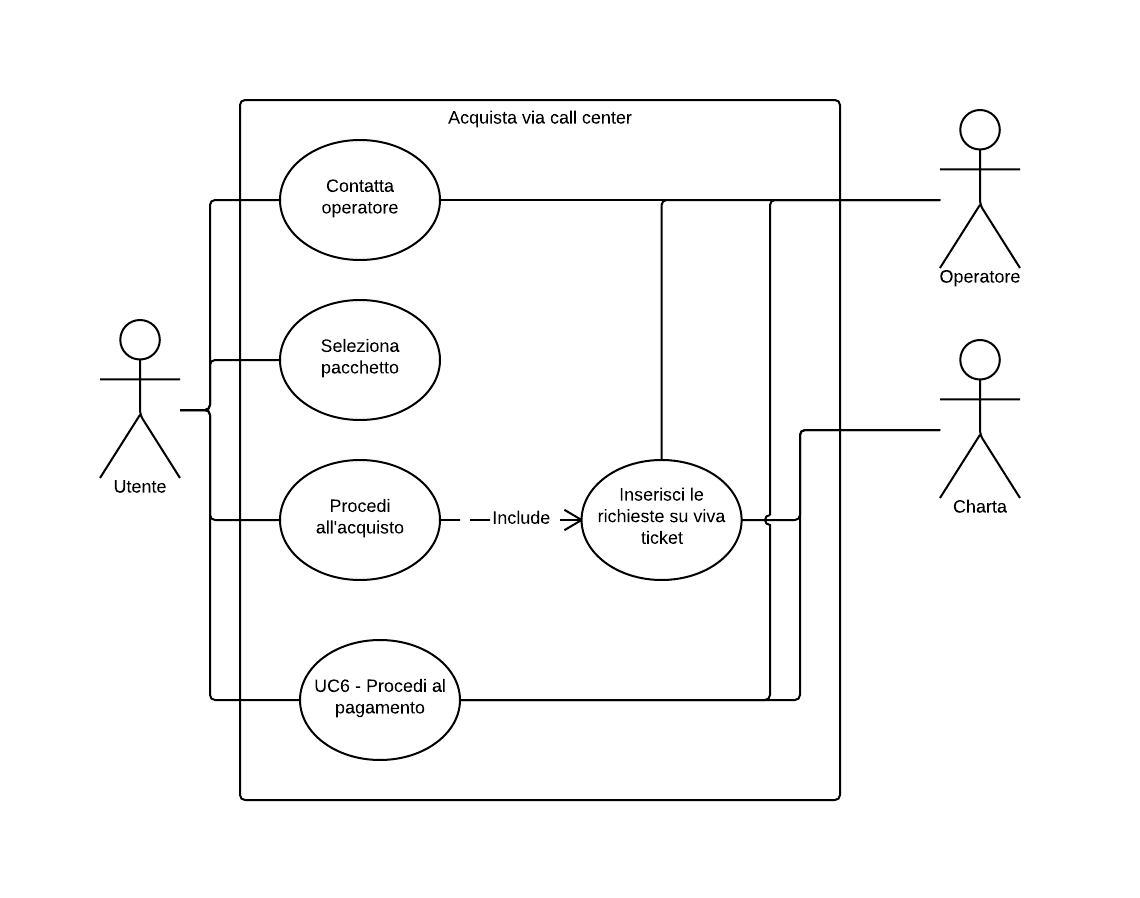
\includegraphics[width=1\textwidth]{images/UC3.png}
\caption{Caso d'uso UC3: Acquisto via call center}
\end{figure}
\begin{itemize}
\item \textbf{Attori:} Utente, operatore, \charta;
\item \textbf{Descrizione:} L'utente contatta il call center, e gli operatori guideranno l'utente nella scelta di uno dei pacchetti disponibili. Quando l'utente ha deciso l'operatore prenota su \tlite acquistando un biglietto a 0 euro. L'ultima operazione per poter ricevere le PadovaCard è il pagamento, descritto in \ref{UC6}.
\item \textbf{Precondizione:} L'utente desidera comprare una o più padova card;
\item \textbf{Flusso principale degli eventi:}
	\begin{itemize}
		\item L'utente chiama il call center;
		\item L'utente, guidato dall'operatore sceglie quale pacchetto acquistare;
        \item L'operatore procede all'eventuale prenotazione della visita alla \cappella;
        \item L'operatore, su OSS, inserisce i dati dell'utente e della PadovaCard.
	\end{itemize}
\item \textbf{Postcondizione:}L'utente deve solamente pagare per completare l'acquisto.
\end{itemize}

\subsubsection{Caso d'uso UC4: Acquisto via IAT}\label{UC4}
\begin{figure}[H]
\centering
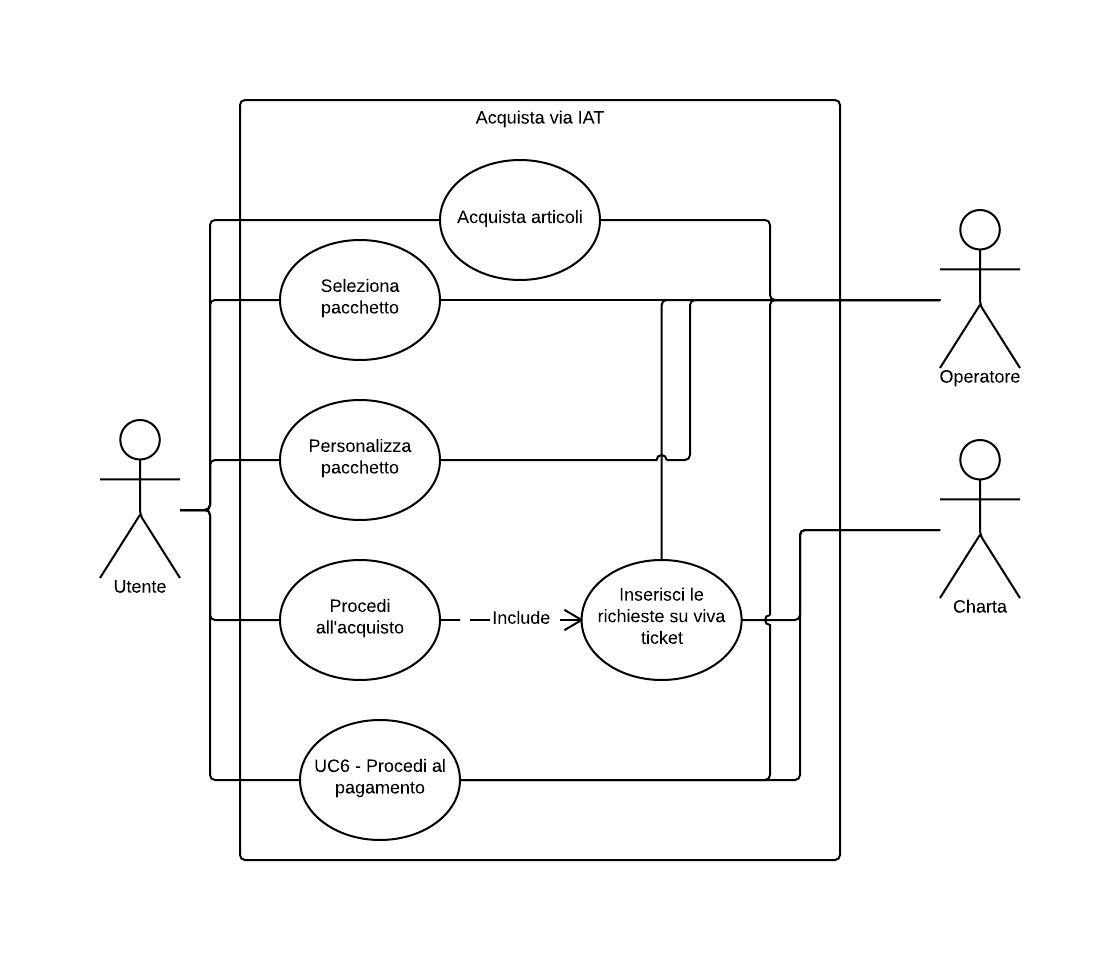
\includegraphics[width=1\textwidth]{images/UC4.png}
\caption{Caso d'uso UC4: Acquisto via IAT}
\end{figure}
\begin{itemize}
\item \textbf{Attori:} Utente, operatore, \charta;
\item \textbf{Descrizione:} L'utente si reca ad uno sportello IAT dove potrà acquistare uno degli articoli in vendita e/o una o più PadovaCard. L'operatore completerà prenota su \tlite acquistando un biglietto a 0 euro, quindi può personalizzare i pacchetti con le preferenze di visita  dell'utente. A questo punto all'utente non resta che pagare quanto acquistato con un unico pagamento, tale operazione è illustrata nella Sezione \ref{UC6}.
\item \textbf{Precondizione:} L'utente desidera comprare una o più padova card;
\item \textbf{Flusso principale degli eventi:}
	\begin{itemize}
    	\item L'utente sceglie un pacchetto;
        \item L'operatore procede alla prenotazione su \tlite;
		\item L'utente assieme all'operatore personalizza il pacchetto;
		\item L'utente può acquistare altri articoli in vendita allo IAT.
	\end{itemize}
\item \textbf{Postcondizione:}L'utente deve solamente pagare per completare l'acquisto.
\end{itemize}

\subsubsection{Caso d'uso UC5: Acquisto via hotel}\label{UCF5}
\begin{figure}[H]
\centering
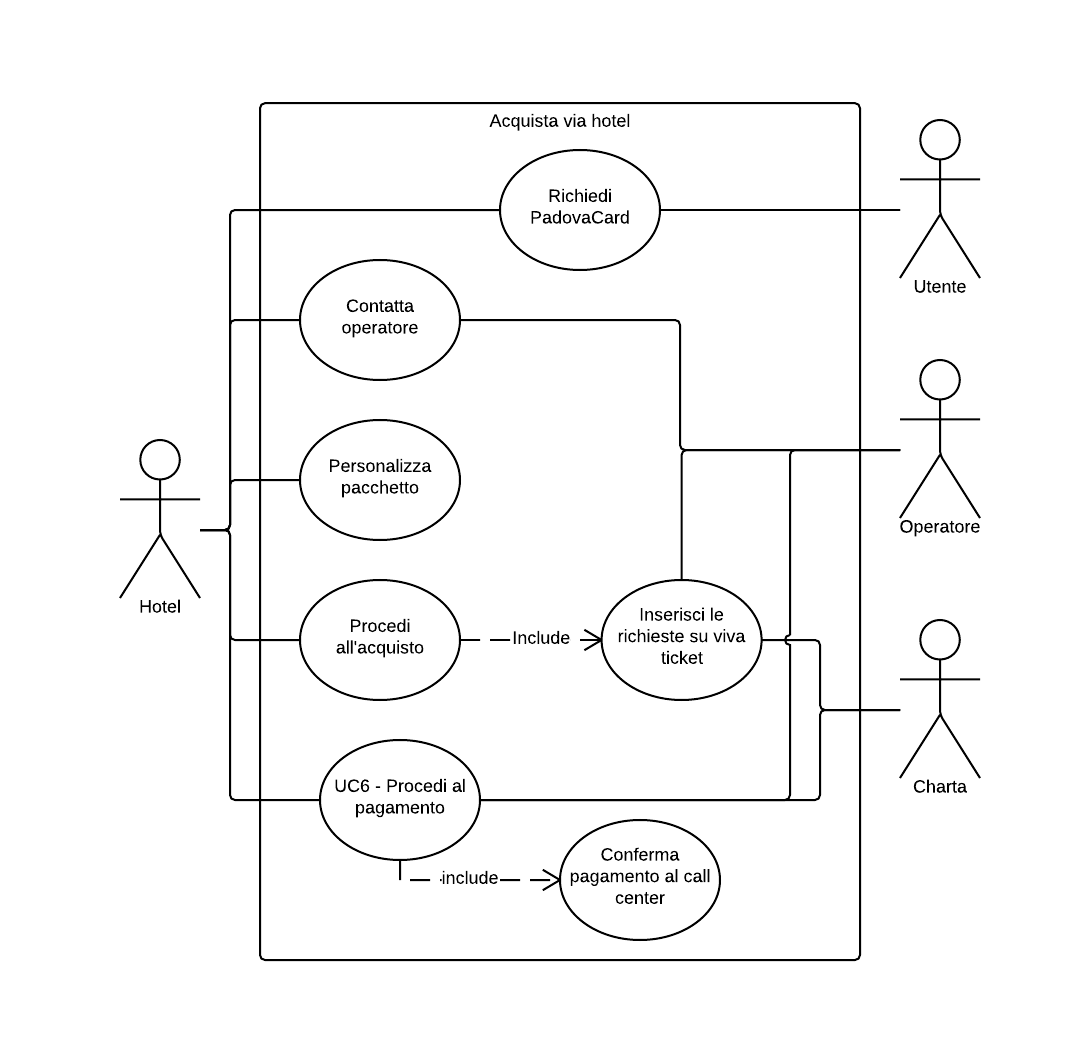
\includegraphics[width=1\textwidth]{images/UC5.png}
\caption{Caso d'uso UC5: Acquisto via hotel}
\end{figure}
\begin{itemize}
\item \textbf{Attori:} Utente, operatore, \charta, hotel;
\item \textbf{Descrizione:} L'utente riferisce ad un membro del personale dell'hotel (se quest'ultimo è convenzionato con PadovaCard) che desidera acquistare una o più PadovaCard. Il personale dell'hotel comunicherà con il call center tramite un canale a priorità maggiore di quello comune, per i dettagli vedere il caso d'uso UC3 alla Sezione \ref{UC3}. Dunque il processo è identico all'acquisto via call center se non che l'hotel fa da intermediario;
\item \textbf{Precondizione:} L'utente desidera comprare una o più padova card;
\item \textbf{Flusso principale degli eventi:}
	\begin{itemize}
    	\item L'utente riferisce all'hotel che desidera comprare una o più PadovaCard;
		\item L'hotel chiama il call center;
		\item L'hotel comunica la data di visita e quale pacchetto acquistare;
        \item L'operatore procede alla prenotazione su \tlite;
        \item Si procede al pagamento.
	\end{itemize}
\item \textbf{Postcondizione:}L'utente deve solamente pagare per completare l'acquisto;
\end{itemize}

\subsubsection{Caso d'uso UC6: Pagamento}\label{UC6}
\begin{figure}[H]
\centering
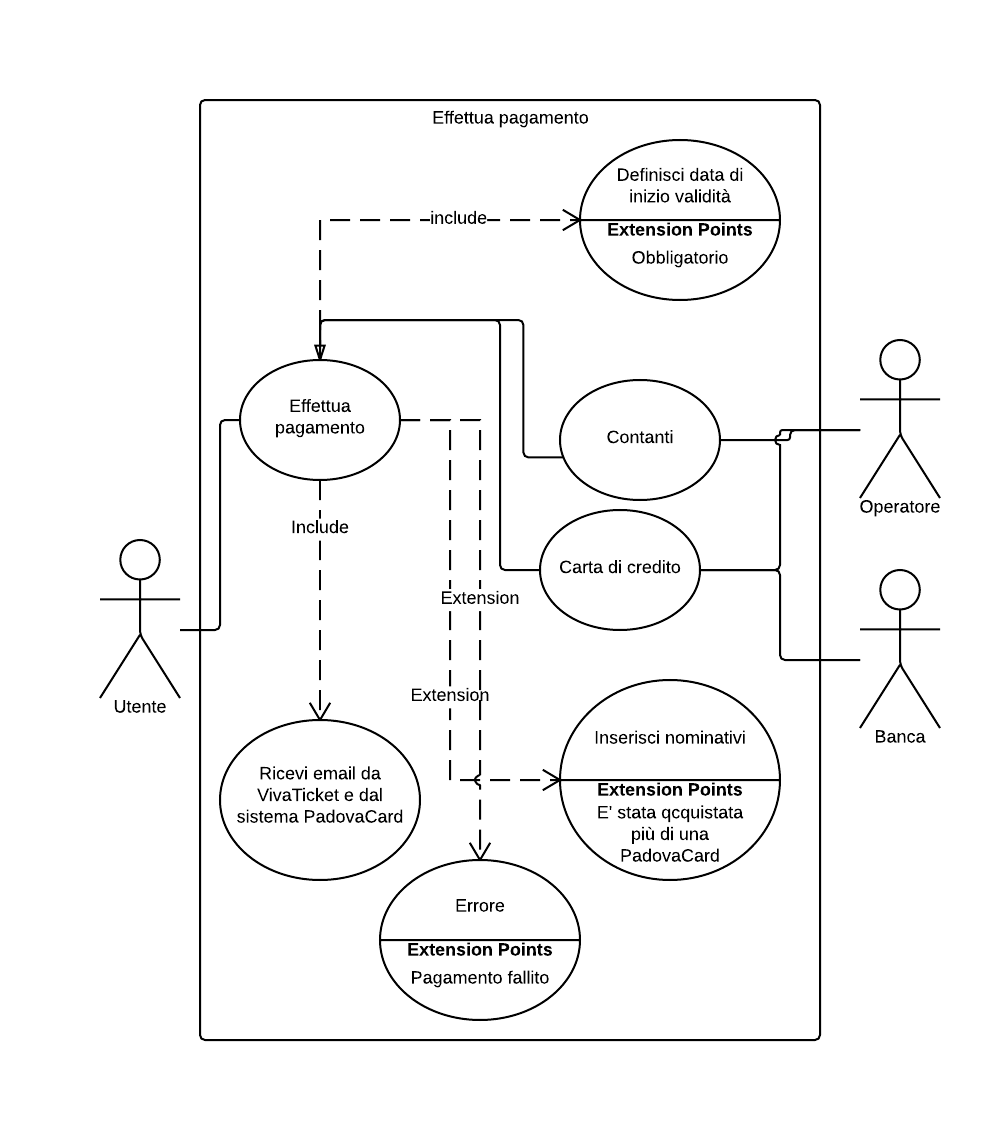
\includegraphics[width=1\textwidth]{images/UC6.png}
\caption{Caso d'uso UC6: Pagamento}
\end{figure}
\begin{itemize}
\item \textbf{Attori:} Utente, operatore, banca;
\item \textbf{Descrizione:} L'utente ha selezionato la propria PadovaCard con uno dei possibili metodi, e si appresta a pagare. E' possibile farlo sempre tramite carta di credito, mentre è possibile  in contanti solo se l'acquisto è stato fatto presso uno sportello IAT\textsuperscript{1}  e via bonifico solo dal call center. Qualora il pagamento andasse a buon fine l'utente riceverà un'unica mail dal sistema con il codice della PadovaCard e il codice di prenotazione \tlite. Qualora durante un'ordine siano acquistate più PadovaCard sarà necessario inserire un nominativo per ognuna di esse, avvalendosi di un operatore. Nel caso in cui l'acquisto avvenga via internet ciò non è possibile, ma una possibile soluzione è proposta come requisito facoltativo alla Sezione \ref{UCF3}.
Fondamentale è poi definire una data e un ora di inizio validità per la PadovaCard (la scadenza si fisserà di conseguenza), tenendo presente che se compresa, la visita alla cappella degli Scrovegni deve essere all'interno del periodo di validità.\\
\begin{footnotesize}
\textit{\textsuperscript{1} Un hotel a sua discrezione potrebbe far pagare l'utente in contanti e poi utilizzare la propria carta di credito}
\end{footnotesize}
\item \textbf{Precondizione:} L'utente ha selezionato il pacchetto da acquistare;
\item \textbf{Flusso principale degli eventi:}
	\begin{itemize}
		\item L'utente paga, via carta di credito, contanti o bonifico;
        \item L'utente stabilisce la data e l'ora di inizio del periodo di validità;
		\item L'utente riceve la mail contenente il codice della PadovaCard.
	\end{itemize}
    \item \textbf{Flusso alternativo degli eventi:}
	\begin{itemize}
    	\item Il pagamento non va a buon fine, la carta è rifiutata dalla banca o l'utente non ha abbastanza contanti;
		\item L'utente acquista più di una PadovaCard, è necessario inserire i nominativi per ognuna.
	\end{itemize}
\item \textbf{Postcondizione:} L'utente ha ricevuto la PadovaCard.
\end{itemize}

\subsubsection{Caso d'uso UC7: Stampa/ristampa tessera}
\begin{figure}[H]
\centering
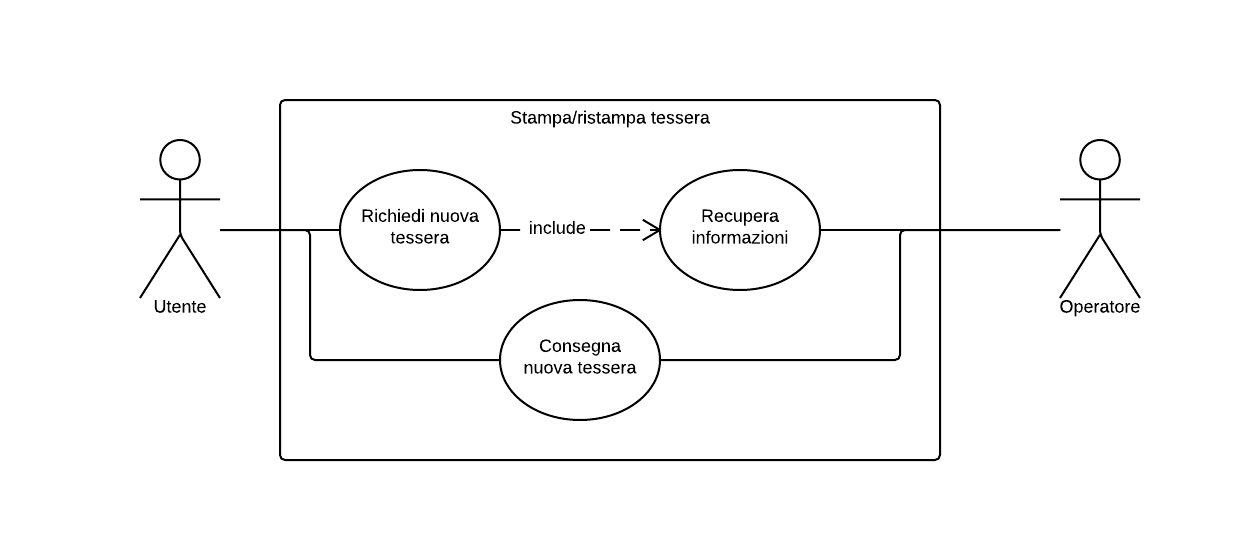
\includegraphics[width=1\textwidth]{images/UC7.png}
\caption{Caso d'uso UC7: Stampa/ristampa tessera}
\end{figure}
\begin{itemize}
\item \textbf{Attori:} Utente, operatore;
\item \textbf{Descrizione:} L'utente si reca ad uno sportello IAT e comunica la propria volontà di avere la propria PadovaCard stampata. Ricordiamo che avere la PadovaCard stampata non è strettamente necessario, in quanto è sufficiente stampare il codice ricevuto via email su carta o mostrare il codice a schermo. L'operatore recupera il codice della PadovaCard partendo dal nominativo dell'utente ed esegue la stampa;
\item \textbf{Precondizione:} L'utente desidera avere stampata la propria PadovaCard, o ha smarrito quella in suo possesso;
\item \textbf{Flusso principale degli eventi:}
	\begin{itemize}
    	\item L'utente desidera la PadovaCard stampata;
        \item L'operatore recupera il codice della PadovaCard;
        \item L'operatore stampa la PadovaCard.
    \end{itemize}
\item \textbf{Postcondizione:}  L'utente ottiene la PadovaCard stampata;
\end{itemize}

\subsubsection{Caso d'uso UC8: Visita struttura}
\begin{figure}[H]
\centering
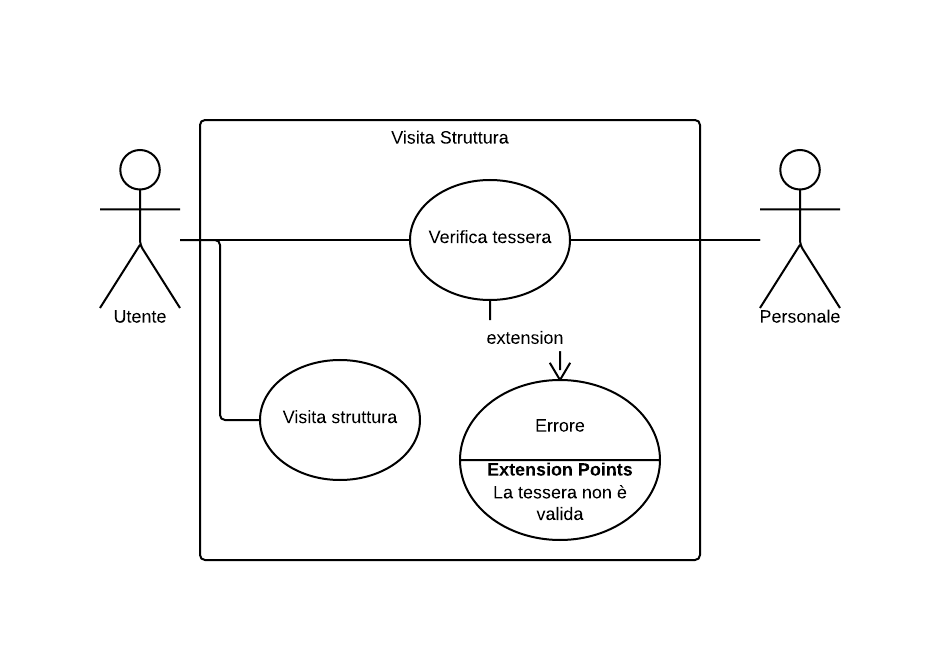
\includegraphics[width=1\textwidth]{images/UC8.png}
\caption{Caso d'uso UC8: Visita struttura}
\end{figure}
\begin{itemize}
\item \textbf{Attori:} Utente, personale;
\item \textbf{Descrizione:} Un utente munito della propria PadovaCard si reca alla struttura che desidera visitare, il personale, autenticato nel sistema legge il codice a barre (stampato o a schermo) tramite l'apposito lettore e visualizza quindi sul monitor se l'utente può visitare la struttura o meno;
\item \textbf{Precondizione:} L'utente vuole visitare una struttura, il personale è autenticato;
\item \textbf{Postcondizione:}  L'utente ha visitato la struttura;
\end{itemize}


\subsubsection{Caso d'uso UC9: Login}
\begin{figure}[H]
\centering
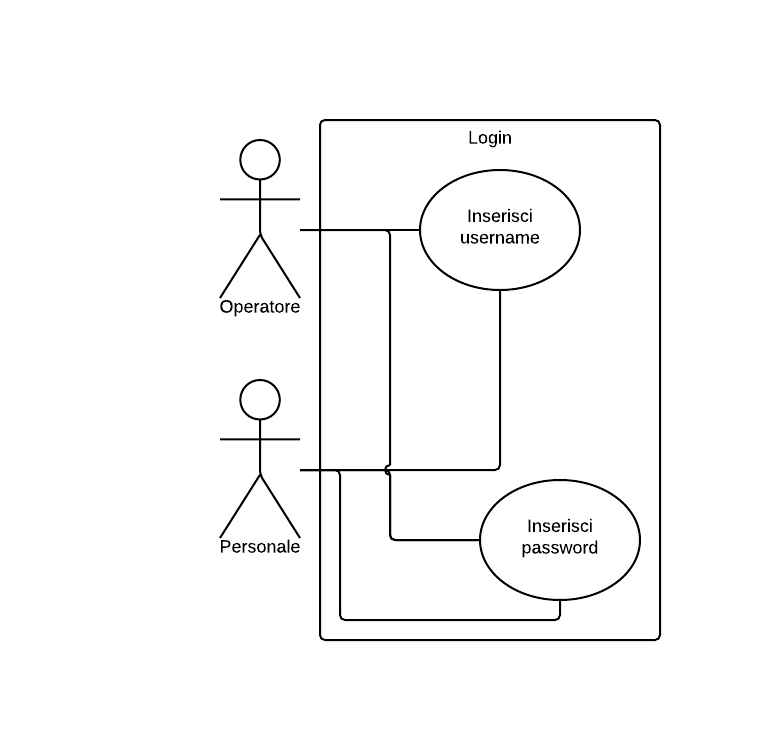
\includegraphics[width=1\textwidth]{images/UC9.png}
\caption{Caso d'uso UC9: Login}
\end{figure}
\begin{itemize}
\item \textbf{Attori:} Personale, operatore;
\item \textbf{Descrizione:} Vengono inserite le credenziali, username e password e se corretti si viene autenticati. Deve poter essere possibile recuperare e modificare la propria password;
\item \textbf{Precondizione:} Il personale e gli operatori non sono autenticati;
\item \textbf{Postcondizione:}  Il personale e gli operatori sono autenticati.
\end{itemize}

\subsubsection{Caso d'uso UCF: Operazioni ad alto livello}\label{UCF}
Il seguente diagramma mostra una visione ad alto livello dei casi d'uso facoltativi. Ogni caso d'uso è analizzato nel dettaglio nelle sezioni successive. I casi d'uso obbligatori si trovano dalla Sezione \ref{UC} in poi.
\begin{figure}[H]
\centering
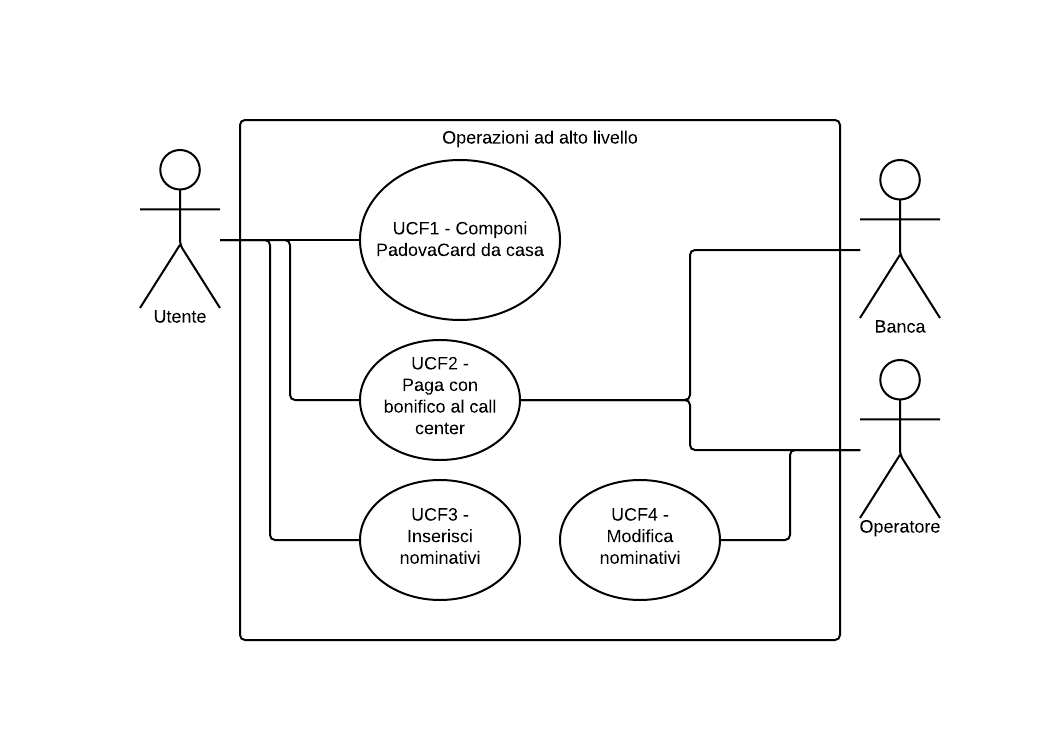
\includegraphics[width=1\textwidth]{images/UCF.png}
\caption{Caso d'uso UCF: Operazioni ad alto livello}
\end{figure}

\subsubsection{Caso d'uso UCF1: Componi PadovaCard da casa}
Questo requisito permette all'utente di personalizzare la propria PadovaCard da casa.
\begin{figure}[H]
\centering
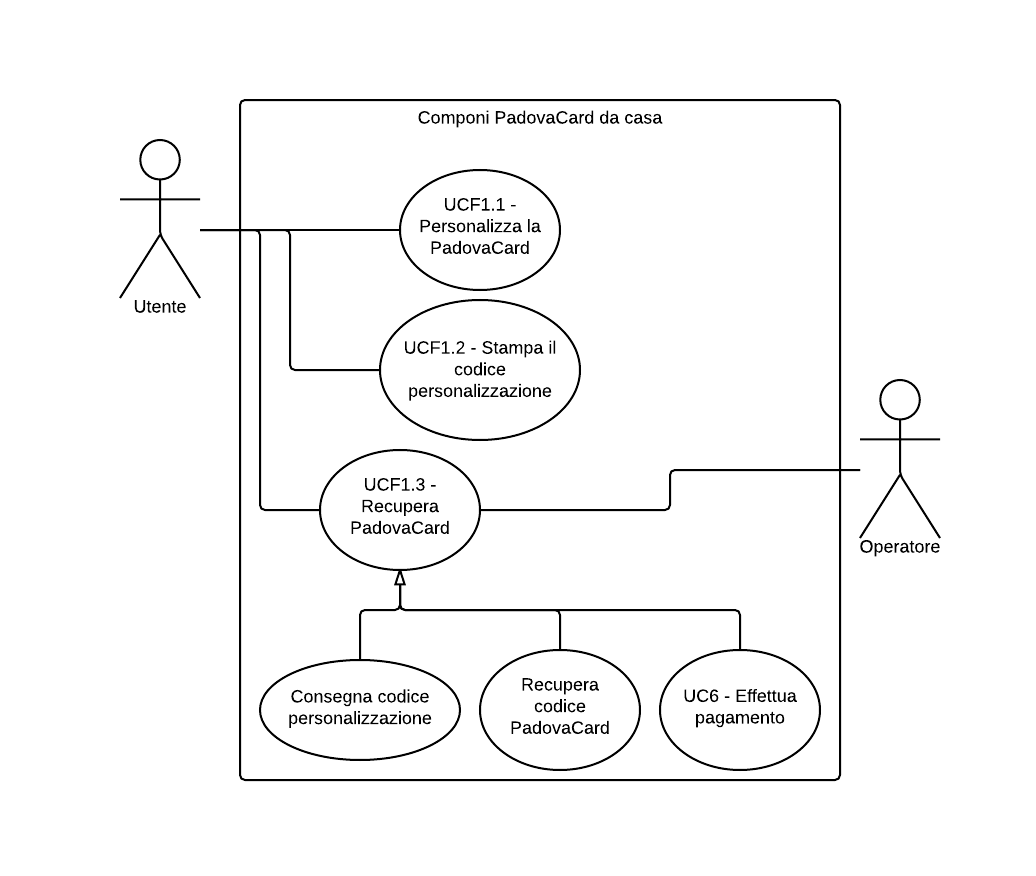
\includegraphics[width=1\textwidth]{images/UCF1.png}
\caption{Caso d'uso UCF1:  Componi PadovaCard da casa}
\end{figure}
\textbf{UCF1.1}
\begin{itemize}
\item \textbf{Attori:} Utente;
\item \textbf{Precondizione:} L'utente accede al portale;
\item \textbf{Descrizione:} L'utente tramite il portale web ha la possibilità di comporre la propria Padovacard;
\item \textbf{Postcondizione:} L'utente ha personalizzato la propria PadovaCard.
\end{itemize}

\textbf{UCF1.2}
\begin{itemize}
\item \textbf{Attori:} Utente;
\item \textbf{Precondizione:} L'utente ha personalizzato la propria PadovaCard;
\item \textbf{Descrizione:} Il portale genera un codice di personalizzazione. Tale codice non è da confondere con quello della PadovaCard, esso infatti non permette di accedere alle strutture;
\item \textbf{Postcondizione:} L'utente è in possesso di un codice di personalizzazione.
\end{itemize}

\textbf{UCF1.3}
\begin{itemize}
\item \textbf{Attori:} Utente, operatore;
\item \textbf{Precondizione:} L'utente è in possesso di un codice di personalizzazione;
\item \textbf{Descrizione:} L'utente con il proprio codice di personalizzazione si reca ad uno sportello IAT, dove l'operatore, leggendo il codice ed interrogando il sistema verrà a conoscenza di come l'utente desidera la propria PadovaCard e questo permette di velocizzarne la creazione. Da questo momento in poi il procedimento è lo stesso di UC4, visibile alla Sezione \ref{UC4}.

\item \textbf{Postcondizione:} L'utente è in possesso della PadovaCard.
\end{itemize}

\subsubsection{Caso d'uso UCF2: Acquisto via internet}
\begin{figure}[H]
\centering
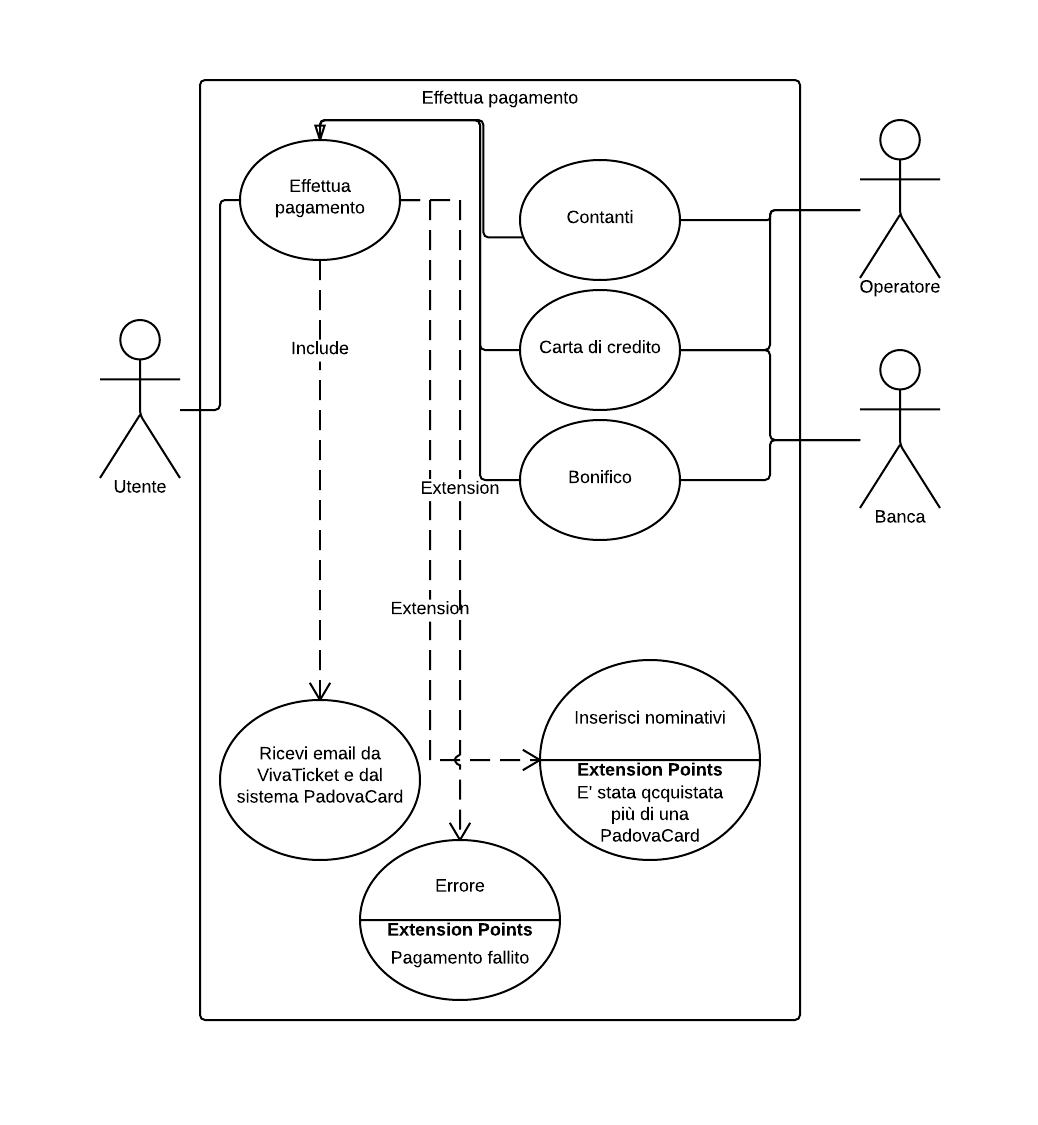
\includegraphics[width=1\textwidth]{images/UCF2.png}
\caption{Caso d'uso UCF2: Acquisto via internet}
\end{figure}
\begin{itemize}
\item \textbf{Attori:} Utente, \charta;
\item \textbf{Descrizione:} L'utente si collega alla piattaforma \vivaticket, direttamente o reinderizzato dal portale descritto in \ref{UC1}. Come già ora accade esso completerà l'operazione su \vivaticket. L'ultima operazione per poter ricevere le PadovaCard è il pagamento, descritto in \ref{UC6}.
\item \textbf{Precondizione:} L'utente desidera comprare una o più padova card;
\item \textbf{Flusso principale degli eventi:}
	\begin{itemize}
		\item L'utente si collega a \vivaticket;
		\item L'utente seleziona il pacchetto desiderato.
	\end{itemize}
\item \textbf{Postcondizione:} L'utente deve solamente pagare per completare l'acquisto.
\end{itemize}

\subsubsection{Caso d'uso UCF3: Inserisci nominativi}\label{UCF3}

\begin{figure}[H]
\centering
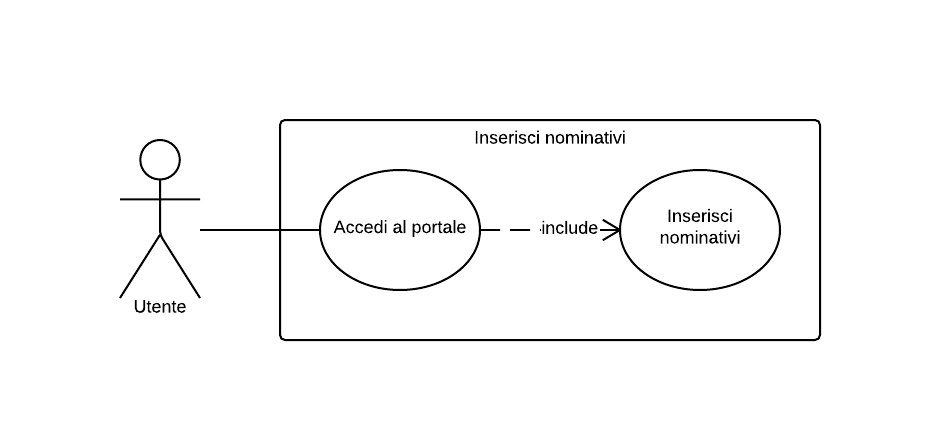
\includegraphics[width=1\textwidth]{images/UCF3.png}
\caption{Caso d'uso UCF3: Inserisci nominativi}
\end{figure}
\begin{itemize}
\item \textbf{Attori:} Utente;
\item \textbf{Descrizione:} Di fronte ad un ordine di più PadovaCard si pone il problema dei nominativi ad esse correlati, come descritto in UC6 - Pagamento (Sezione \ref{UC6}). Per ovviare al problema nel caso in cui l'utente abbia effettuato l'ordine via internet è possibile rendere disponibile una funzionalità che permette all'utente stesso di inserire i nominativi, accedendo al sistema con il codice dell'ordine effettuato su \vivaticket e compilando i form che gli vengono presentati.
\item \textbf{Precondizione:} L'utente è in possesso di più PadovaCard;
\item \textbf{Postcondizione:}  L'utente ha collegato un nominativo per ogni PadovaCard in suo possesso.
\end{itemize}

\subsubsection{Caso d'uso UCF4: Modifica nominativi}
Non è presente un diagramma UML in quanto si tratta di un caso d'uso semplicissimo.
\begin{itemize}
\item \textbf{Attori:} Operatore;
\item \textbf{Descrizione:} Assumendo che l'utente abbia inserito i nominativi, come descritto in UCF3, Sezione \ref{UCF3}, deve essere possibile modificarli, in caso di errore. Se si da tale possibilità all'utente c'è il rischio che ne approfitti per associare diversi proprietari ad un unica PadovaCard, anche se non contemporaneamente. 
L'utente che vuole modificare tali nominativi dovrà quindi contattare un operatore e richiedere la modifica.
\item \textbf{Precondizione:} L'utente ha inserito i nominativi per ogni Padovacard del suo ordine;
\item \textbf{Postcondizione:} L'operatore ha modificato uno o più nominativi.
\end{itemize}

\subsubsection{Caso d'uso UCF6: Creazione utente}
\begin{figure}[H]
\centering
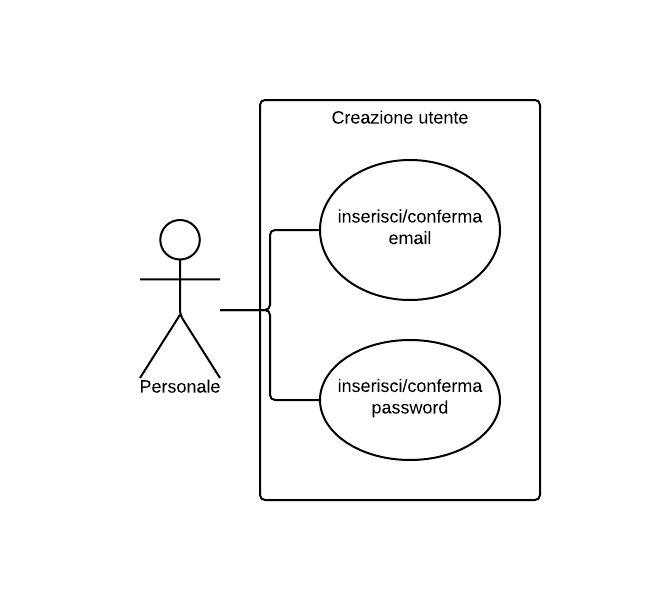
\includegraphics[width=1\textwidth]{images/UCF6.png}
\caption{Caso d'uso UCF6: Creazione utente}
\end{figure}

\begin{itemize}
\item \textbf{Attori:} Personale;
\item \textbf{Descrizione:} Il personale delle strutture deve poter creare il proprio account su OSS;
\item \textbf{Precondizione:} Il membro del personale non possiede un account su OSS;
\item \textbf{Postcondizione:} Il membro del personale possiede un account su OSS.
\end{itemize}

\subsection{Requisiti}
Ogni requisito è identificato da un codice, che segue il seguente formalismo:

\begin{center}
\textbf{R\{X\}\{Y\} \{Gerarchia\}}
\end{center}

Dove:
\begin{itemize}
\item X corrisponde alla priorità del requisito e può assumere i seguenti valori:
	\begin{itemize}
		\item O = Obbligatorio;
        \item F = Facoltativo o opzionale.
	\end{itemize}
\item Y corrisponde al sistema di riferimento e può assumere i seguenti valori:
	\begin{itemize}
		\item O = Operatore, si tratta di operatori degli sportelli IAT o del call center;
        \item U = Utente, si tratta del fruitore della PadovaCard, tipicamente un turista;
        \item P = Personale, si tratta del personale dei luoghi d'interesse convenzionati con PadovaCard;
        \item S = Sistema, si tratta del sistema che si occupa della gestione della PadovaCard.
	\end{itemize}
\item Gerarchia identifica la relazione gerarchica che c'è tra i requisiti di uno stesso tipo. C'è quindi una struttura gerarchica per ogni tipologia di requisito.
\end{itemize}

\newpage

\def\arraystretch{2}
\begin{center}
\begin{longtable}[H]{| p{.20\textwidth} | p{.60\textwidth} | p{.20\textwidth}|}
\hline 
Requisito & Descrizione & Fonti \\ \hline
ROU 1 & L'utente deve poter consultare online le offerte relative alla propria padova card  & UC1 \\ \hline
ROU 2 & L'utente, tramite operatore deve poter comunicare i nominativi associati ad ogni tessera, se su \tlite ne è stata acquistata più di una all'interno di un solo ordine. & UC6 \\ \hline
ROU 3 & L'utente può acquistare uno degli n pacchetti preconfigurati chiamando il call center, pagando con carta di credito o bonifico e ricevere via mail il codice. & UC3, UC6 \\ \hline
ROU 4 & L'utente può acquistare uno degli n pacchetti preconfigurati in uno degli alberghi convenzionati pagando con carta di credito o bonifico e riceve via mail il codice, e opzionalmente un \glossario{voucher} cartaceo. & UC5, UC6 \\ \hline
ROU 5 & L'utente può acquistare uno degli n pacchetti preconfigurati, o comporre il proprio ad uno sportello IAT, pagando con carta di credito o contanti e riceverà la tessera ed eventualmente il codice via mail.  & UC4, UC6 \\ \hline
ROU 6 & L'utente può accedere alla struttura solo se è prevista all'interno della sua PadovaCard, se essa non è scaduta (superato il periodo di validità) e se non ha già effettuato la visita.  & UC8 \\ \hline
ROU 7 & L'utente può farsi stampare una nuova tessera in caso essa venga smarrita. (L'utente è comunque in possesso del codice su email).  & UC7 \\ \hline
RFU 8 & L'utente deve inserire autonomamente la data e l'ora di inizio validità della PadovaCard.  & UC6 \\ \hline
RFU 9 & L'utente può acquistare uno degli n pacchetti preconfigurati su \vivaticket pagando con carta di credito e ricevere via mail il codice. & UCF2, UC6 \\ \hline
RFU 10 & L'utente può comporre la propria PadovaCard, visualizzando in tempo reale prezzi ed offerte dei vari pacchetti/ingressi.  & UCF1.1, UCF1.2, UCF1.3 \\ \hline
RFU 11 & L'utente può stampare un codice relativo alla propria composizione ed acquistarla ad uno sportllo IAT.  & UCF1.2, UCF1.3 \\ \hline
RFU 13 & L'utente, tramite il portale deve poter inserire i nominativi associati ad ogni tessera, se su vivaticket ne è stata acquistata più di una all'interno di un solo ordine.  & UCF3 \\ \hline
ROP 14 & Il personale deve loggarsi al sistema con un id univoca.  & UC9 \\ \hline
ROP 15 & Il personale deve poter recuperare la propria password in caso di smarrimento.  & UC9 \\ \hline
ROP 16 & Il personale deve poter modificare la propria password.  & UC9 \\ \hline
ROP 17 & Il personale avrà un lettore di codici che rileverà il codice presente sulla tessera, sul \glossario{voucher} o a a schermo, nel caso in cui l'utente utilizzi la mail su cellulare.  & UC8 \\ \hline
RFP 18 & Il personale deve poter creare un account su OSS & UCF6 \\ \hline
ROO 19 & Gli operatori devono loggarsi al sistema con un id univoca.  & UC9 \\ \hline
ROO 20 & Gli operatori devono poter recuperare la propria password in caso di smarrimento.  & UC9 \\ \hline
ROO 21 & Gli operatori devono poter modificare la propria password.  & UC9 \\ \hline
ROO 22 & Gli operatori potranno selezionare su \tlite un biglietto di costo zero.  & UC4, UC3 \\ \hline
ROO 23 & L'operatore dovrà poter inserire nel sistema i nominativi associati alle padovacard se queste sono state acquistate su \tlite tramite un unico ordine.  & UC6 \\ \hline
ROO 24 & Gli operatori IAT effettuano un unico pagamento nel caso in cui vengano combinati l'acquisto di una o più padova card sia con i pacchetti predefiniti sia personalizzate e altri articoli in vendita (mappe, guide, souvenir etc.). & UC6 \\ \hline
ROO 25 & Gli operatori possono modificare, su richiesta dell'utente il periodo di validità di una Padovacard già acquistata. & UC2 \\ \hline
ROS 26 & Il sistema partendo dai dati ricevuti da \tlite genererà un codice univoco per ogni tessera e vi associerà tutte le informazioni, per poi salvarle nel database.  &  \\ \hline
ROS 27 & Allo scadere del periodo di validità il sistema marca il codice della carta come non più valida. &  \\ \hline
ROS 28 & Quando si effettua una visita il sistema marca tale visita non più effettuabile da parte di quel codice.  &  \\ \hline
ROS 29 & Il sistema mantiene separati i dati relativi alle PadovaCard da tutti gli altri, ma raggruppa i dati sulle vendite, per cui la vendita di una PadovaCard è salvata assieme a qualunque altra vendita, ma nessuna informazione è fornita su tale padovaCard se non il codice.  &  \\ \hline
RFS 31 & Il sistema riconosce come non valida una tessera a cui non è associato un nominativo. &  \\ \hline
RFO 31 & Gli operatori devono poter modificare i nominativi di un ordine già pagato. & UCF4 \\ \hline
\caption{Tabella requisiti}
\end{longtable}
\end{center}


\section{Progettazione}\label{progettazione}
\subsection{Base di dati}
OSS possiede una propria base di dati formata da 19 tabelle e 5 viste. Si vogliono mantenere logicamente separati i dati relativi alla PadovaCard.\\

Di seguito venogno riportati lo schema concettuale, lo schema logico e il DDL dell'espansione del database, mentre non viene riportata la struttura del database esistente in quanto non interagirà con le nuove tabelle.\\

Una nota sui nomi delle tabelle è d'obbligo, CackePHP richiede l'utilizzo di una sintassi standard per i nomi delle tabelle, necessaria per effettuare l'accoppiamento model-tabella. Risulta quindi necessario utilizzare nomi inglesi plurali o nomi italiani che terminano per s.
\subsubsection{Modello concettuale}
\begin{figure}[H]
\centering
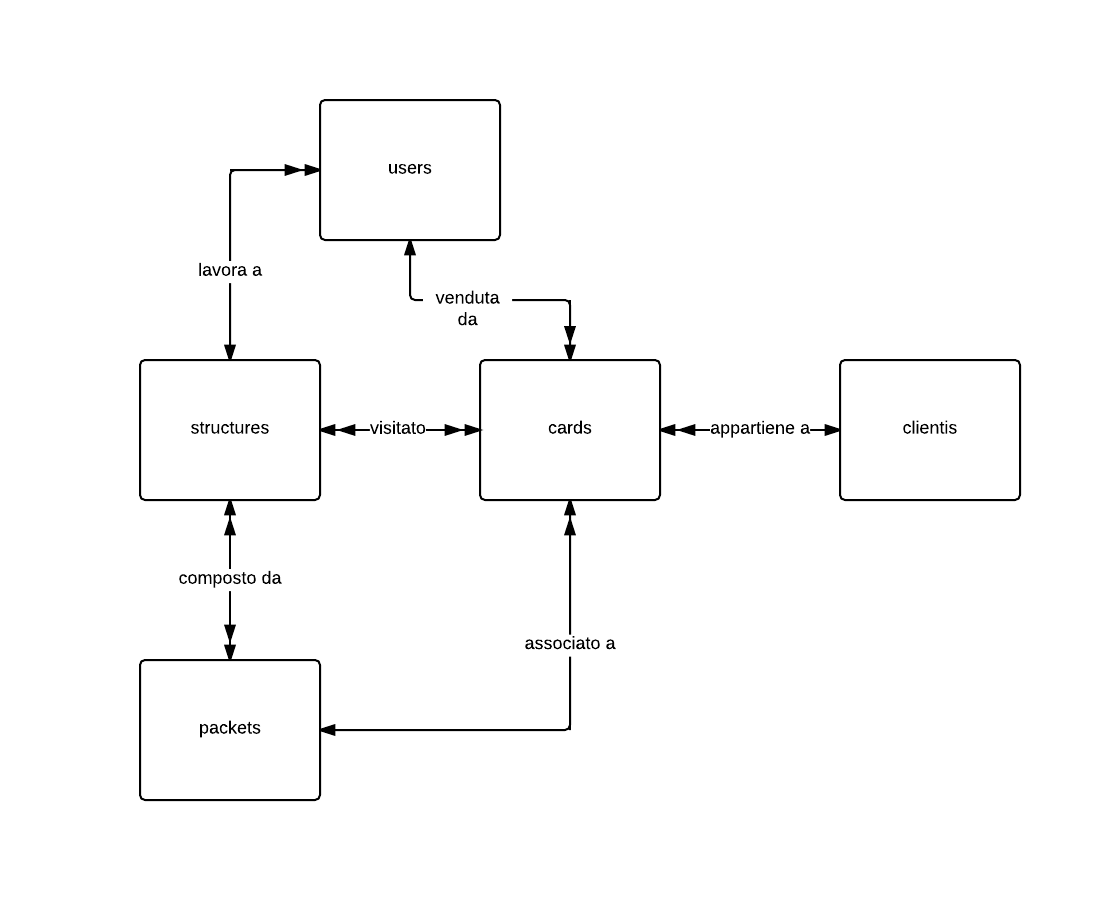
\includegraphics[width=1\textwidth]{images/concettuale.png}
\caption{Modello concettuale della base di dati}
\end{figure}
L'espansione del database già esistente si compone di 3 tabelle, cards, packets e structures mentre clientis e users sono già presenti.
Le nuove tabelle saranno collegate al database esistente tramite clientis e users utilizzando chiavi esterne.\\ \\
\textbf{Tabelle}
\begin{itemize}
\item \textbf{card:} contiene tutte le informazioni sulle PadovaCard;
\item \textbf{clientis:} contiene l'anagrafica degli utenti che hanno acquistato una PadovaCard o altri articoli che necessitano di anagrafica dal sistema;
\item \textbf{packets:} contiene i dati relativi ai pacchetti associabili alla PadovaCard. Ricordiamo che un pacchetto è un insieme di strutture visitabili;
\item \textbf{structures:} contiene i dati su tutte le strutture convenzionate con PadovaCard;
\item \textbf{users:} contiene i dati relativi agli operatori e al personale delle strutture. In futuro potrebbe contenere anche quelli relativi agli hotel.
\end{itemize}
\textbf{Relazioni}
\begin{itemize}
\item \textbf{appartiene a:} cards è connessa con una relazione uno a molti a clientis perchè ogni utente può avere una sola PadovaCard attiva, ma più di una non attive, ogni Padovacard attiva deve essere connessa ad un cliente, mentre quelle inattive possono non esserlo. Questa distinzione si rende necessaria per quando in futuro gli utenti potranno acquistare via web le PadovaCard. Ci sarà un periodo di tempo tra la creazione della carta e l'inserimento di tutti i nominativi a causa degli ordini di più PadovaCard. Escludendo questo requisito anche le PadovaCard inattive hanno un nominativo associato
\item \textbf{associata a:} cards è connessa con una relazione uno a molti a packets perchè ad ogni PadovaCard è associato un solo pacchetto di strutture, mentre un pacchetto può essere associato a più Padovacard;
\item \textbf{composto da:} packets è collegato con una relazione molti a molti a structures in quanto ogni pacchetto è formato da più strutture ed ogni struttura può essere presente su più pacchetti;
\item \textbf{lavora a:} users è collegato con una relazione uno a molti a strcutures per mantenere i dati relativi al personale delle strutture;
\item \textbf{venduta da:} cards è connessa con una relazione uno a molti ad users in quanto bisogna tener traccia di quale operatore vende una PadovaCard, una Padovacard può essere venduta da un solo operatore e un operatore può vendere più PadovaCard. Una carta può non essere venduta da un operatore, nel caso in cui l'acquisto sia fatto via internet;
\item \textbf{visitato:} cards è connesso con una relazione molti a molti a strutture perchè è necessario tener traccia di quali struttre ha visitato l'utente per impedire che con la stessa PadovaCard venga visitata più volte la stessa struttura.


\end{itemize}


\subsubsection{Modello logico-relazionale}\label{logicorelazionale}

\begin{figure}[H]
\centering
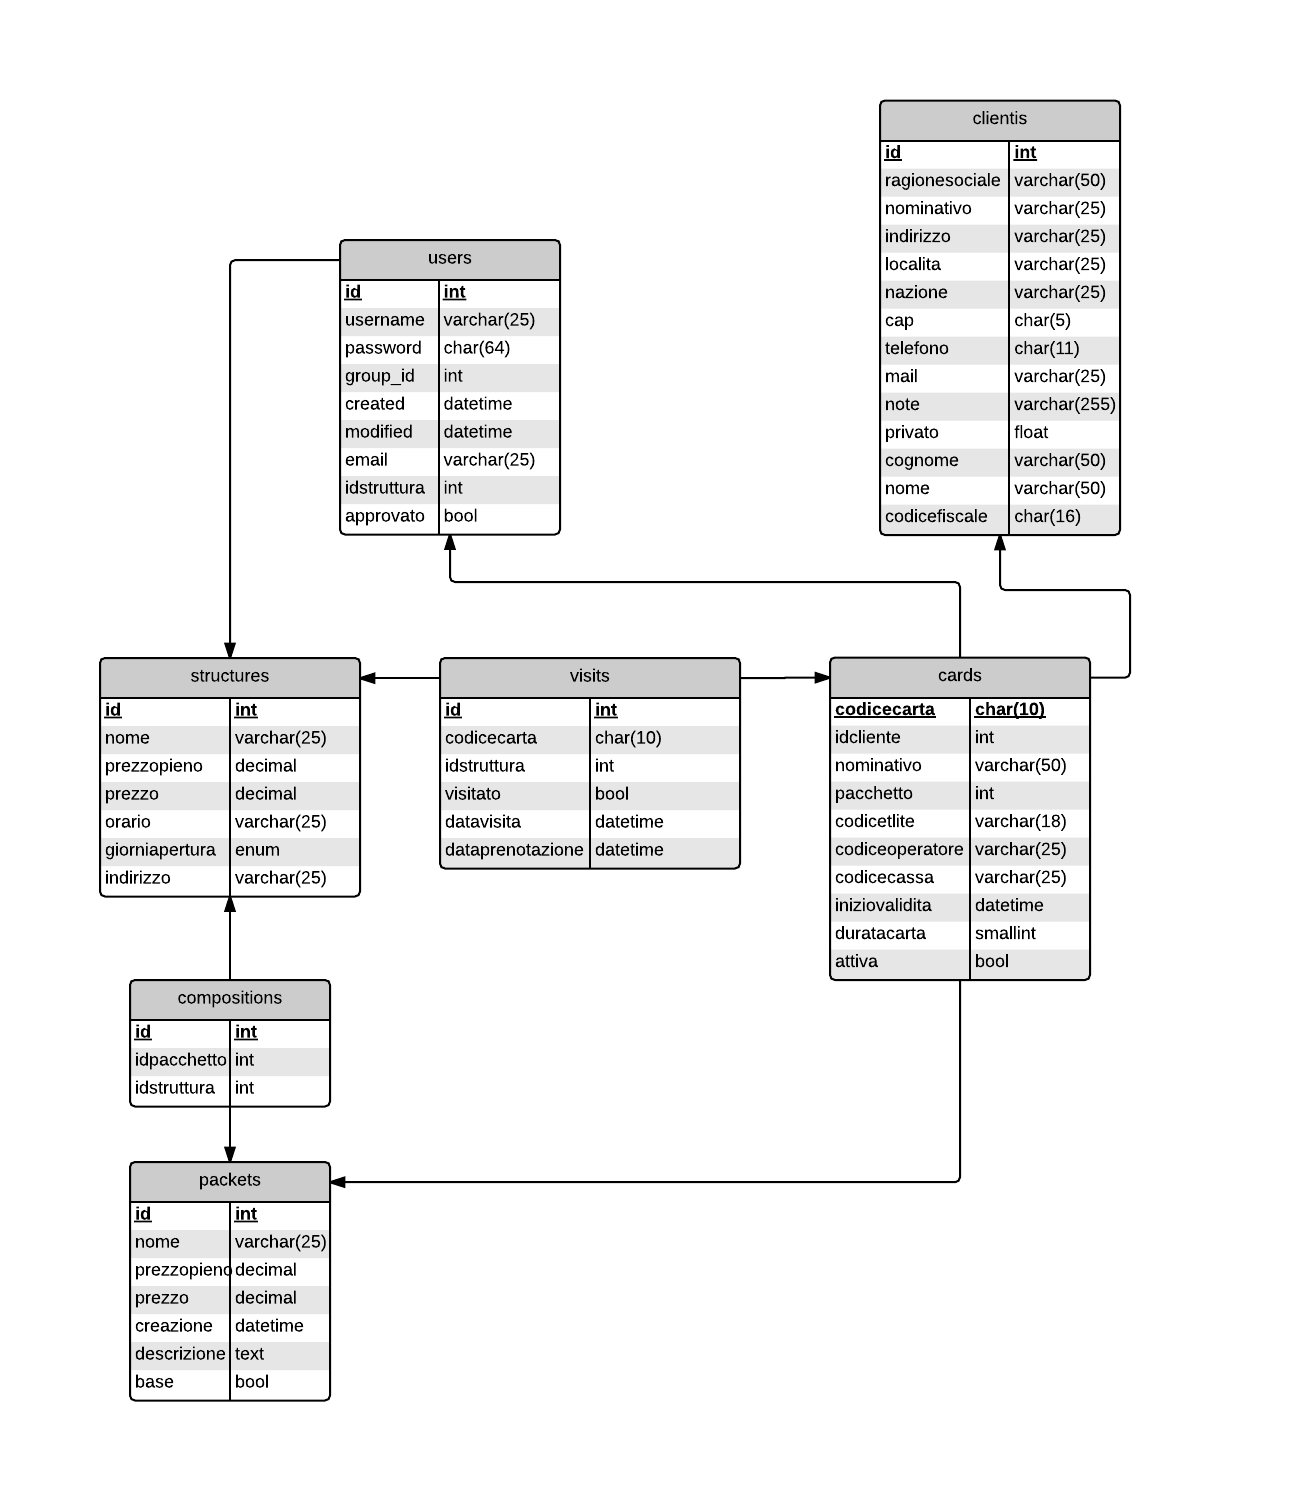
\includegraphics[width=1\textwidth]{images/logico.png}
\caption{Modello logico della base di dati}
\end{figure}
CakePHP prevede che ogni tabella abbia una sola chiave primaria in quanto non supporta chiavi primarie composite, per questo è necessario aggiungere una chiave primaria "di servizio" per CakePHP in tabelle come visite e composizione.\\ \\
\textbf{Note di progettazione}\\ \\
Inizialmente cards conteneva un campo dal nome prenotazionecappella, di tipo datetime, che doveva contenere la data e l'ora della prenotazione alla \cappella. \'E stato deciso di spostare tale campo sulla tabella visits e rinominarlo dataprenotazione. Questo permette di gestire la prenotazione a più strutture nel caso in cui in futuro ci sia tale necessità. \'E altresi vero che la maggior parte dei record avrà Null come valore di dataprenotazione, ma essendo questo di tipo datetime si è stimato uno spreco di memoria nel caso peggiore di meno di 3 Megabyte annui. Il calcolo è il seguente:
Dimensione di datetime $*$ numero stimato di PadovaCard vendute in un anno $*$ numero massimo di strutture per pacchetto = $8byte*20000*15 $. \\

Attualmente per le password vengono usati campi di tipo char(40) ovvero un campo che può contenere fino ad un massimo di 40 caratteri, sufficienti a contenere l'output della funziona hash \glossario{MD5}. Il tirocinante propone di utilizzare un campo char(64) in previsione dell'utilizzo dell'hash \glossario{SHA256}. Tale cambio è motivato nella Sezione \ref{hash}. \\

Nella tabella users è presente un campo username di tipo varchar(255). Nonostante varchar occupi solamente lo spazio per i caratteri effettivamente scritti, quando vengono create le tabelle temporanee durante le query viene allocata la lunghezza massima. Per questo il tirocinante propone di modificare varchar(255) in varchar(25), più che sufficiente per i valori di tale campo. \\

Clientis contiene i campi cap, telefono e note di tipo varchar(25). Il tirocinante propone di modificare il tipo di cap in char(5), telefono in char(11) e note in varchar(255) in quanto tale valore per varchar è il massimo ottenibile con un solo byte di overhead. Codicefiscale che ora ha tipo varchar(16) viene modificato in tipo char(16). \\

La chiave primaria di cards è codicecarta, con tipo char(10). Si è scelto di utilizzare codicecarta e non un id auto increment in quanto è univoca e permette di evitare una join durante la lettura di visits. Questo è ottimale in quanto visits sarà la tabella con più query in lettura, mentre si stima la perdita di efficienza nell'uso di char invece di int inferiore al 20\% nel caso peggiore, considerando la lunghezza del char, il fatto che è indicizzato e che il motore usato è \glossario{INNODB}. \\

Sempre in cards duratacarta è uno samllint. Ad oggi sono previste solo due durate, 48 e 72 ore, per cui un tipo bool sarebbe stato sufficiente ma uno smallint permette di creare più di due tipologie di durata. \\

La tabella packets contiene il campo descrizione di tipo text, ritenuto necessario se si vuole salvare qui la descrizione completa della struttura che apparirà nel sito che l'utente adrà a consultare per ottenere le informazioni sulla PadovaCard. \\

Cards contiene il flag attiva che indica se la carta è stata pagata, e se è quindi valida. Questo flag è settato subito a 1 se il pagamento avviene con contanti o carta di credito, mentre viene posto a 0 in attesa del pagamento con bonifico. \\

Cards contiene un campo nominativo e un campo idcliente. Idcliente viene utilizzato per collegare la PadovaCard all'anagrafica di chi ha effettuato l'ordine, che può essere una persona sia fisica che giuridica. Nominativo contiene il nome del proprietario della PadovaCard e sarà il nome presente nel voucher. Per questo motivo ci potranno essere più PadovaCard attive con lo stesso idcliente mentre il nominativo sarà unico.\\

Per i campi che rappresentano denaro è stato utilizzato il tipo decimal e si è deciso di continuare ad utilizzarlo in quanto non presenta rischi di approssimazione che invece ha il tipo float. \\ \\
\textbf{Tabelle}\\ \\
Nella seguente Sezione verranno descritte nel dettaglio le tabelle che saranno create. Per ogni tabella è fornita una descrizione sul contenuto e un elenco dei suoi campi, comprensivo di tipo e altre note. \\ \\
PK indica che tale campo è \glossario{chiave primaria} della tabella. \\
FK indica che tale campo  è \glossario{chiave esterna} della tabella.\\
\\ \\
CARDS: Contiene tutti i dati relativi alla PadovaCard.
\begin{itemize}
\item codicecarta: varchar(10) \textit{\textless PK\textgreater}
\item idcliente: int \textit{\textless FK\textgreater}
\item pacchetto: int \textit{\textless FK\textgreater}
\item nominativo: varchar(50)
\item codicetlite: varchar(18)
\item codiceopertatore: varchar(25)
\item codicecassa: varchar(25)
\item iniziovalidita: datetime
\item duratacarta: smallint
\item attiva: bool 
\end{itemize}
CLIENTIS: Contiene l'anagrafice degli utenti.
\begin{itemize}
\item id: int \textit{\textless PK\textgreater}
\item ragionesociale: varchar(50)
\item nominativo: varchar(25)
\item indirizzo: varchar(25)
\item localita: varchar(25)
\item nazione: varchar(25)
\item cap: char(5)
\item telefono: char(11)
\item mail: varchar(25)
\item note: varchar(255)
\item privato: float
\item cognome: varchar(50)
\item nome: varchar(50)
\item codicefiscale: char(16)
\end{itemize}
COMPOSITIONS: Tabella creata dalla relazione "composta da", collega le strutture ai pacchetti.
\begin{itemize}
\item id: int \textit{\textless PK\textgreater}
\item idpacchetto: int \textit{\textless FK\textgreater}
\item idstruttura: int \textit{\textless FK\textgreater}
\end{itemize}
PACKETS: Contiene i dati relativi ai pacchetti, composizioni di strutture visitabili.
\begin{itemize}
\item id: int \textit{\textless PK\textgreater}
\item nome: varchar(25)
\item prezzopieno: decimal
\item prezzo: decimal
\item creazione: datetime
\item descrizione: text
\item base: bool
\end{itemize}
STRUCTURES: Contiene i dati relativi alle strutture convenzionate con PadovaCard.
\begin{itemize}
\item id: int \textit{\textless PK\textgreater}
\item nome: varchar(25)
\item prezzopieno: decimal
\item prezzo: decimal
\item orario: datetime
\item giorniapertura: enum('LU','MA','ME','GI','VE','SA','DO')
\item indirizzo: varchar(25)
\end{itemize}
USERS: Contiene i dati riguardanti gli operatori e il personale delle strutture.
\begin{itemize}
\item id: int \textit{\textless PK\textgreater}
\item username: varchar(25)
\item password: char(64)
\item group\_id: int
\item created: datetime
\item modified: datetime
\item email: varchar(25)
\item idstruttura int \textit{\textless FK\textgreater}
\item approvato: bool
\end{itemize}
VISITS: Tabella creata dalla relazione "visitato", tiene traccia di quali strutture sono state visitate da una data PadovaCard, e di eventuali prenotazioni.
\begin{itemize}
\item id INT \textit{\textless PK\textgreater}
\item codicecarta: varchar(10) \textit{\textless FK\textgreater}
\item idstruttura: int \textit{\textless FK\textgreater}
\item visitato: bool
\item datavisita: datetime
\item dataprenotazione: datetime
\end{itemize}
\textbf{Definizione dello schema logico tramite \glossario{DDL} di MySQL}
\lstset{frame=single}
\begin{center}
\begin{lstlisting}
create table clientis (
  id int(11) not null auto_increment,
  ragionesociale varchar(50) default null,
  nominativo varchar(25) default null,
  indirizzo varchar(25) default null,
  localita varchar(25) default null,
  nazione varchar(25) default null,
  cap varchar(25) default null,
  telefono varchar(25) default null,
  mail varchar(50) default null,
  note varchar(25) default null,
  privato float default null,
  cognome varchar(50) default null,
  nome varchar(50) default null,
  codfiscale varchar(16) default null,
  primary key (id)
) ENGINE=InnoDB  DEFAULT CHARSET=utf8 AUTO_INCREMENT=585;

alter table clientis 
	modify column cap char(5),
    modify column telefono char(11),
    modify column note varchar(255);

create table users (
  id int(11) NOT NULL auto_increment,
  username varchar(255) not null,
  password char(40) not null,
  group_id int(11) not null,
  created datetime default null,
  modified datetime default null,
  PRIMARY KEY  (id)
) ENGINE=InnoDB  DEFAULT CHARSET=utf8 AUTO_INCREMENT=51;

alter table users
	modify column password char(64);
    modify column username varchar(25),
    add email varchar(25),
    add approvato bool,
    add idstruttura int,
    add foreign key (idstruttura) references structures (id);

create table packets(
	id int not null auto_increment,
	nome varchar(25) not null,
    prezzopieno decimal default null,
    prezzo decimal default null,
    creazione datetime default null,
	descrizione text default null,
    base bool default 0,
	primary key (id)
)ENGINE=InnoDB DEFAULT CHARSET=utf8; 
	
create table structures(
	id int not null auto_increment,
    nome varchar(25) not null,
    prezzopieno decimal default null,
    prezzo decimal default null,
    orario varchar(25) default null,
    giorniapertura enum('LU','MA','ME','GI','VE','SA','DO') default null,
    indirizzo varchar(25) default null,
	primary key (id)
)ENGINE=InnoDB DEFAULT CHARSET=utf8;

create table compositions(
	id int not null auto_increment,
    idpacchetto int not null,
    idstruttura int not null,
    primary key (id),
    foreign key (idpacchetto) references packets(id),
    foreign key (idstruttura) references structures(id)
)ENGINE=InnoDB DEFAULT CHARSET=utf8;

create table cards(
codicecarta char(10) not null,
idcliente int not null,
pacchetto int not null,
nominativo varchar(50),
codicetlite varchar(18) not null,
codiceoperatore varchar(25),
codicecassa varchar(25),
iniziovalidita datetime,
duratacarta smallint not null,
attiva bool default 0,
foreign key (idcliente) references clientis(id),
foreign key (pacchetto) references packets(id),
primary key (codicecarta)
)ENGINE=InnoDB DEFAULT CHARSET=utf8;
\end{lstlisting}
\end{center}

\subsection{Architettura del sistema}
Di seguito viene riportata l'architettura di OSS ad alto livello, che si rifà all'architettura MVC imposta da CakePHP. 
Successivamente View, Model e Controller saranno mostrati nel dettaglio con le relative classi. \\

Dopo questa visione d'insieme, nella Sezione \ref{specificacomponenti} per ogni requisito verrànno proposti uno o più diagrammi delle attività e di classe,
ogni  componente progettata viene collegata ad un requisito e ad una classe, il tracciamento completo si trova nella Sezione \ref{tracciamento}.

\begin{figure}[H]
\centering
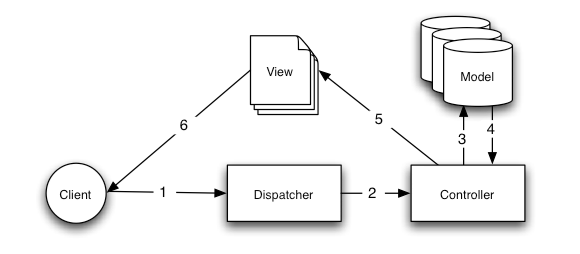
\includegraphics[width=1\textwidth]{images/basic_mvc.png}
\caption{Una tipica richiesta MVC in OSS}
\end{figure}

\begin{figure}[H]
\centering
%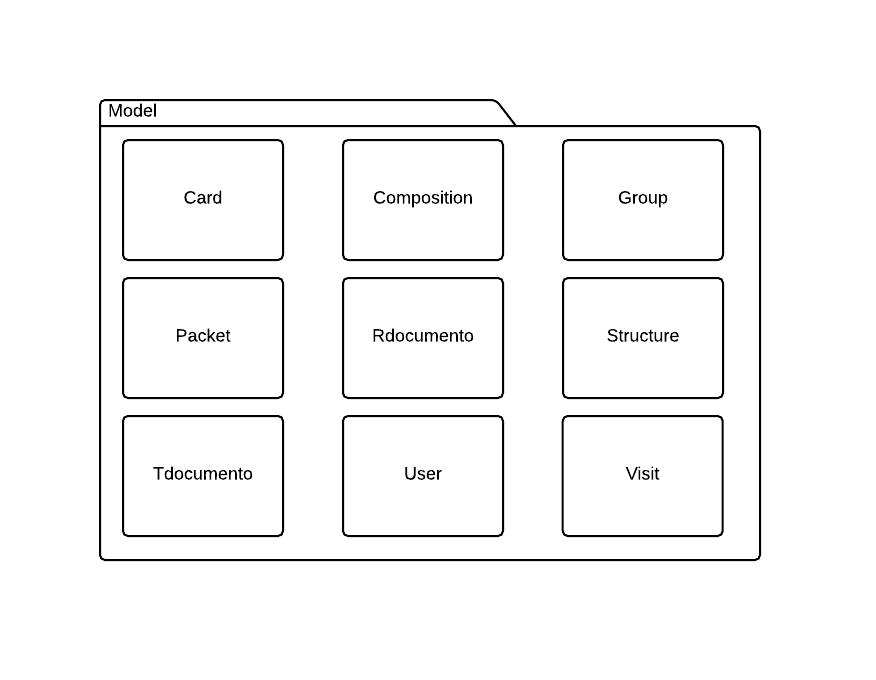
\includegraphics[width=1\textwidth]{images/model.png}
\caption{Pacchetto Model}
\end{figure}

\begin{figure}[H]
\centering
%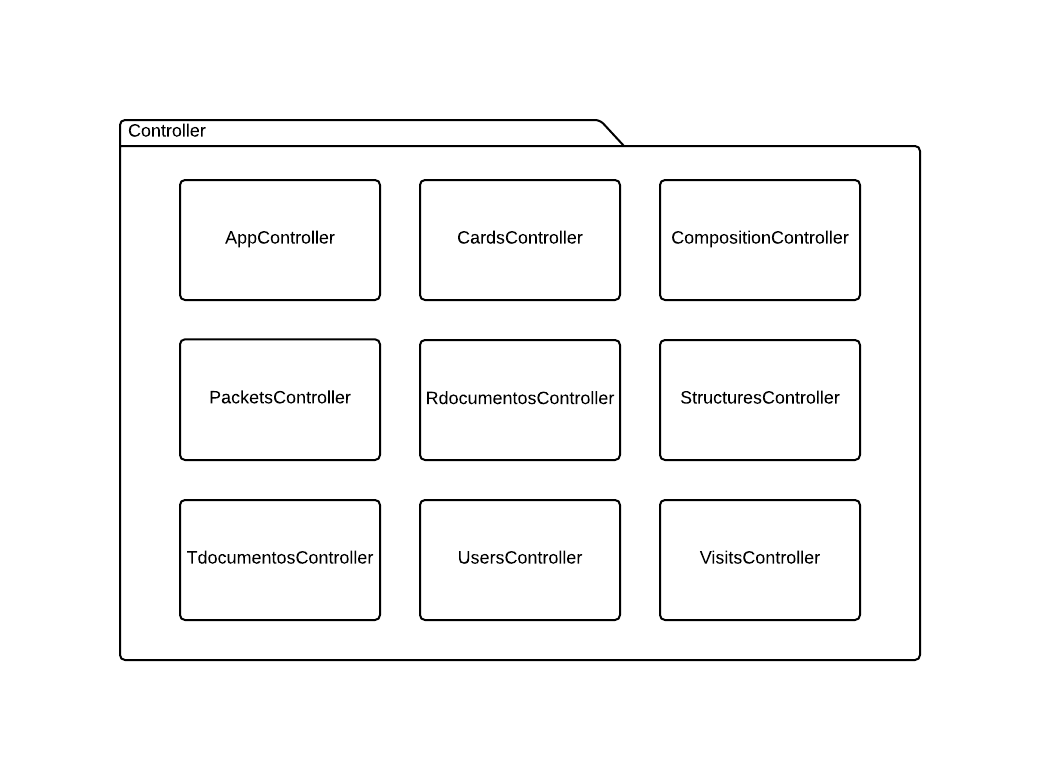
\includegraphics[width=1\textwidth]{images/controller.png}
\caption{Pacchetto Controller}
\end{figure}

\begin{figure}[H]
\centering
%\includegraphics[width=1\textwidth]{images/view.png}
\caption{Pacchetto View}
\end{figure}

\subsection{Funzionamento \tlite}\label{progettazionetlite}
Dalla Figura \ref{tlite} si evince il percorso che l'operatore deve compiere per effettuare la prenotazione. Di particolare interesse è mostrare i punti in cui il nuovo processo differisce da quello attuale:
\begin{itemize}
\item Il biglietto venduto sarà a costo zero, questo permette di concludere la prenotazione anche senza conferma di pagamento;
\item Il resoconto dell'ordine va stampato in formato testuale;
\item \tlite non invia nessuna email all'utente, è da valutare se si vuole inviare una email ad un'apposita casella postale di \net.
\end{itemize}
I punti che invece restano invariati sono:
\begin{itemize}
\item Vi è un solo codice \tlite per ogni prenotazione, indipendentemente dal numero di posti riservati;
\item L'anagrafica del cliente che effettua l'ordina va inserita;
\item \'E necessario annullare manualmente l'ordine nel caso in cui il cliente non concluda il pagamento su OSS.
\end{itemize}

\tlite permette di stampare il resoconto dell'ordine, per ottenere un file invece di una stampa cartacea è sufficiente creare a livello di sistema operativo (Windows) una finta stampante che stampa su file, ed impostare come output un formato testuale in qaunto semplice da \glossario{parsare} su OSS in un momento successivo.

\begin{figure}[H]
\centering
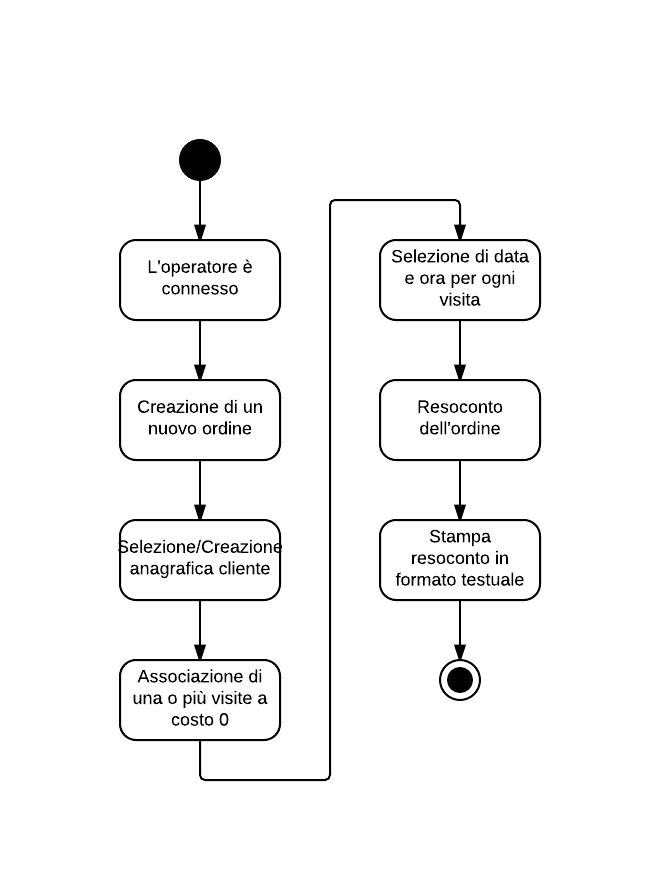
\includegraphics[width=0.8\textwidth]{images/tlite.png}
\caption{Pacchetto View \label{tlite}}
\end{figure}

\subsection{Specifica componenti}\label{specificacomponenti}
\subsubsection{Users}
\def\arraystretch{2}
\begin{table}[H]
\centering
\begin{tabular}{|l|l|}
\hline
Model & User \\ \hline
Controller & UsersControllers \\ \hline
View & Users \\ \hline
Requisiti & ROP 14, ROP 15, ROP 16, RFP 18, ROO 19, ROO 20, ROO 21 \\ \hline
\end{tabular}
\caption{Tracciamento componente-requisiti Users}
\end{table}
Questa componente si occupa della gestione degli utenti, dagli amministratori di OSS agli operatori e con l'estensione di OSS si andrà ad aggiungere anche il personale delle strutture.
Dato che il sistema OSS verrà reso accessibile anche all'esterno della rete \net, si è obbligati a rispettare le direttive sulla privacy, per questo sono stati aggiunti il campo email e il campo approvato nella relativa tabella del database  e la possibilità di recuperare autonomamente la password persa. Vi è inoltre l'obbligo di modificare la password ogni sei mesi in quanto il sistema contiene \glossario{dati personali} (Ma non \glossario{dati sensibili}).
Quest'ultima funzionalità è già implementata.

\begin{table}[H]
\centering
\begin{tikzpicture}
\node (table) [inner sep=0pt] {
\begin{tabular}{l}
  {UsersController} \\
  \hline
  \\
  \hline
  +index(): void \\
  +view(id: string): void  \\
  +add(): void \\
  +edit(id: string): void \\
  +chgpsw(id: string): void \\
  +delete(id: string): void \\
  +login(): void \\
  +logout(): void \\
  +rcvpsw(): void  \\
  +signup(): void  \\
\end{tabular}
};
\draw [rounded corners=.5em] (table.north west) rectangle (table.south east);
\end{tikzpicture}
\caption{Controller:UsersController}
\end{table}



\paragraph{Login}

Il processo di autenticazione esiste già, devono però essere apportate le seguenti modifiche:
\begin{itemize}
\item Nella view va aggiunto un link per il recupero password, che chiamerà il metodo rcvpsw e uno per la registrazione che chiamerà il metodo signup;
\item L'autenticazione dovrà verificare oltre alla corrispondenza username/password anche se tale utente è attivo, controllando se il flag "approvato" è impostato a 1. Questo è possibile farlo aggiungendo l'elemento scope all'array che imposta le opzioni del componente Auth in AppController.php.
\end{itemize}

\label{hash} CakePHP offre la crittazione tramite hash con algoritmo \glossario{MD5}, SHA1, \glossario{SHA256} e blowfish. Attualmete viene utilizzato SHA1. Va tenuto presente però che al momento OSS è un software interno mentre dopo l'espansione verrà reso accessibile anche all'esterno. Per tale motivo il tirocinante suggerisce di passare ad una crittazione più forte come SHA-256, comunque supportata nativamente da CakePHP.

\paragrafo{Diagramma delle attività}

Di seguito è presentato il diagramma delle attività riguardante l'autenticazione a OSS. I soggetti di tali azioni sono operatori e personale.\\

\begin{figure}[H]
\centering
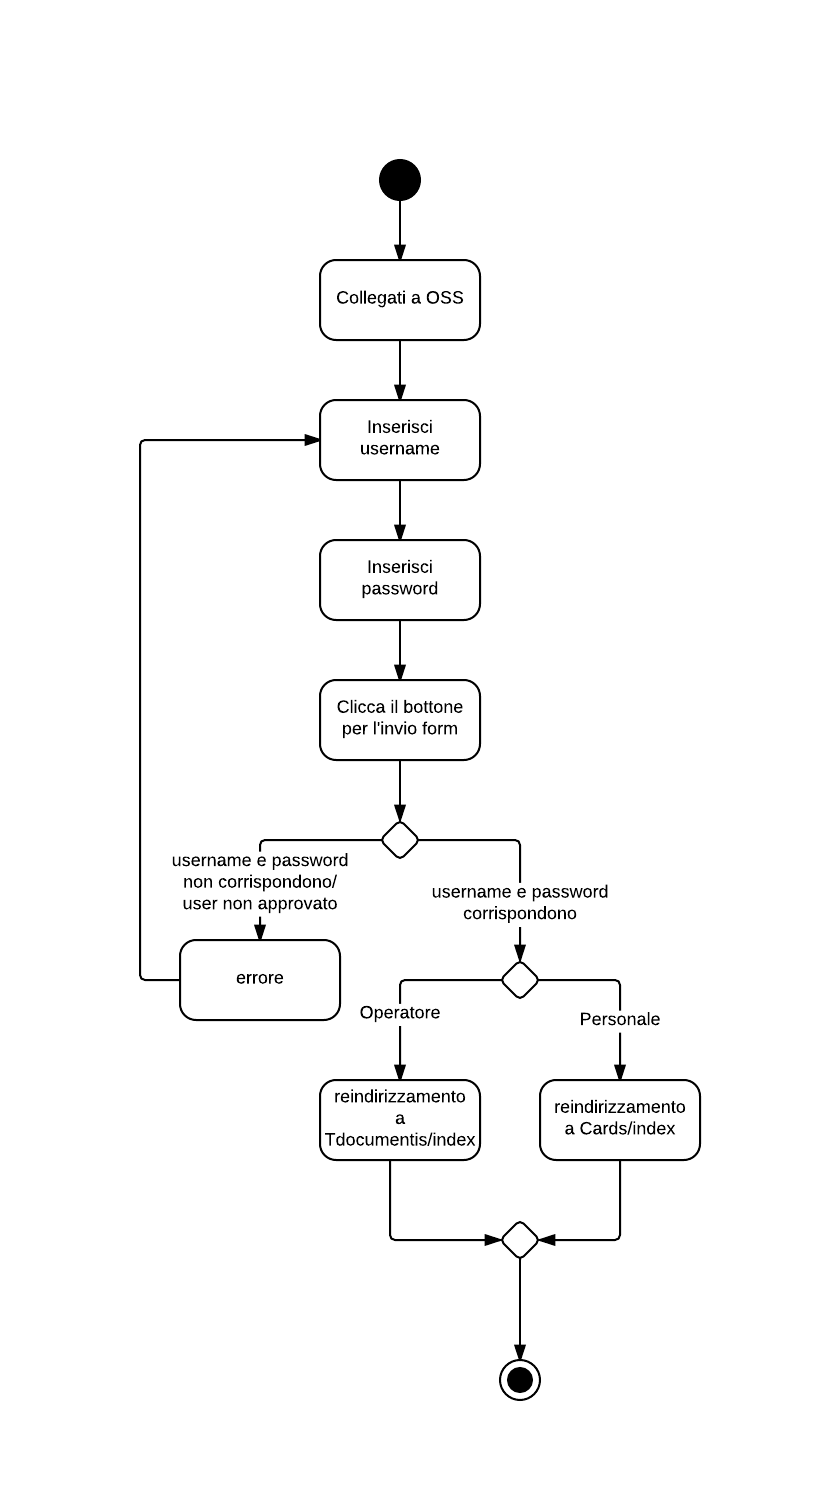
\includegraphics[width=0.8\textwidth]{images/user_login.png}
\caption{Diagramma attività: Login}
\end{figure}

\paragraph{Recupero password}

Il sistema non prevede la possibilità di recupero password, si tratta quindi di una nuova funzionalità. Quando l'utente richiede di recuperare la password:
\begin{itemize}
\item Il sistema genera una passoword casuale di 8 caratteri;
\item Il sistema cripta la passowrd generata con l'algoritmo scelto e salva l'output nel campo password relativo all'utente;
\item Il sistema invia una email con la password all'utente;
\item Nel frattempo l'utente è stato reindirizzato alla pagina di login dove un'avviso gli comunica di controllare la propria casella email;
\item L'utente utilizza la password ricevuta per autenticarsi.
\end{itemize} 

\paragrafo{Diagramma delle attività}
Di seguito è presentato il diagramma delle attività riguardante il recupero password. I soggetti di tali azioni sono operatori e personale.\\


\begin{figure}[H]
\centering
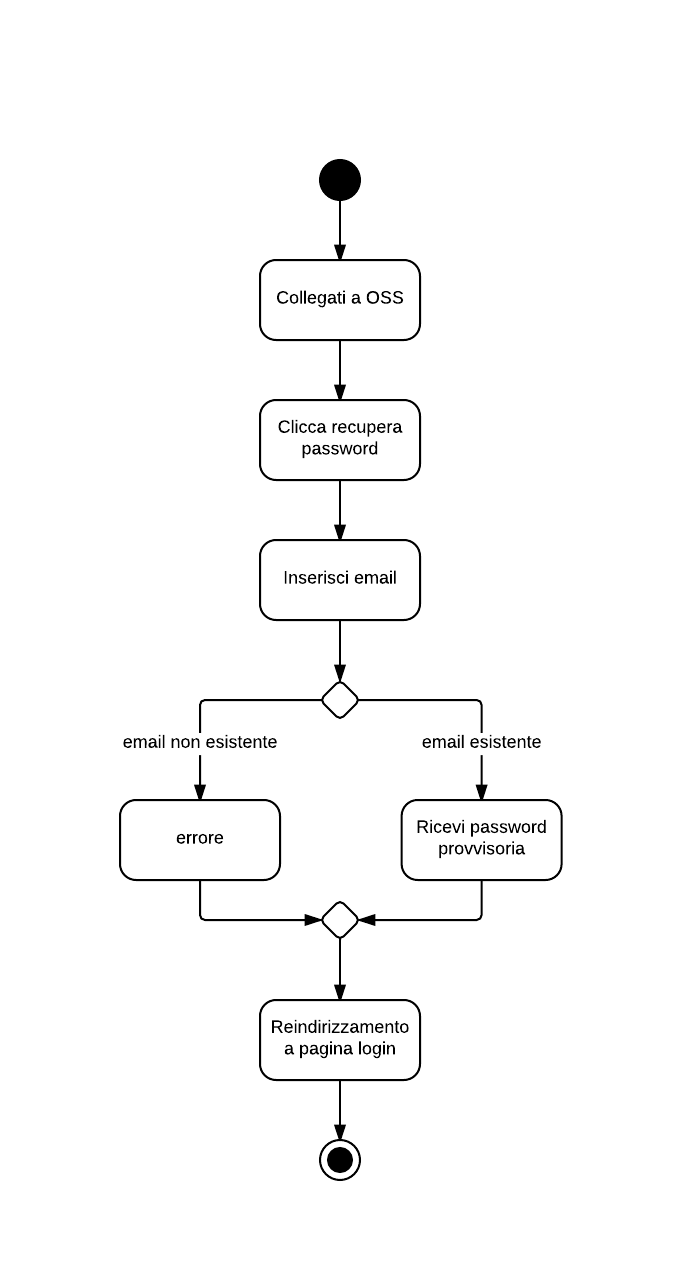
\includegraphics[width=0.6\textwidth]{images/user_rcvpsw.png}
\caption{Diagramma attività: Recupero password}
\end{figure}


\paragraph{Nuovo utente}
Al momento all'interno di OSS sono presente solamente alcuni operatori. Dato che anche il personale delle strutture utilizzerà OSS è necessario che essi possano registrarsi. Non è indicato che sia l'amministratore ad inserirli a sistema in quanto il sistema contiene \glossario{dati sensibili} e dunque la password deve essere conosciuta solo dal proprietario del profilo.

\paragrafo{Diagramma delle attività}
Di seguito è presentato il diagramma delle attività riguardante la creazione di un nuovo utente. I soggetti di tali azioni sono personale e l'amministratore di OSS.\\

\begin{figure}[H]
\centering
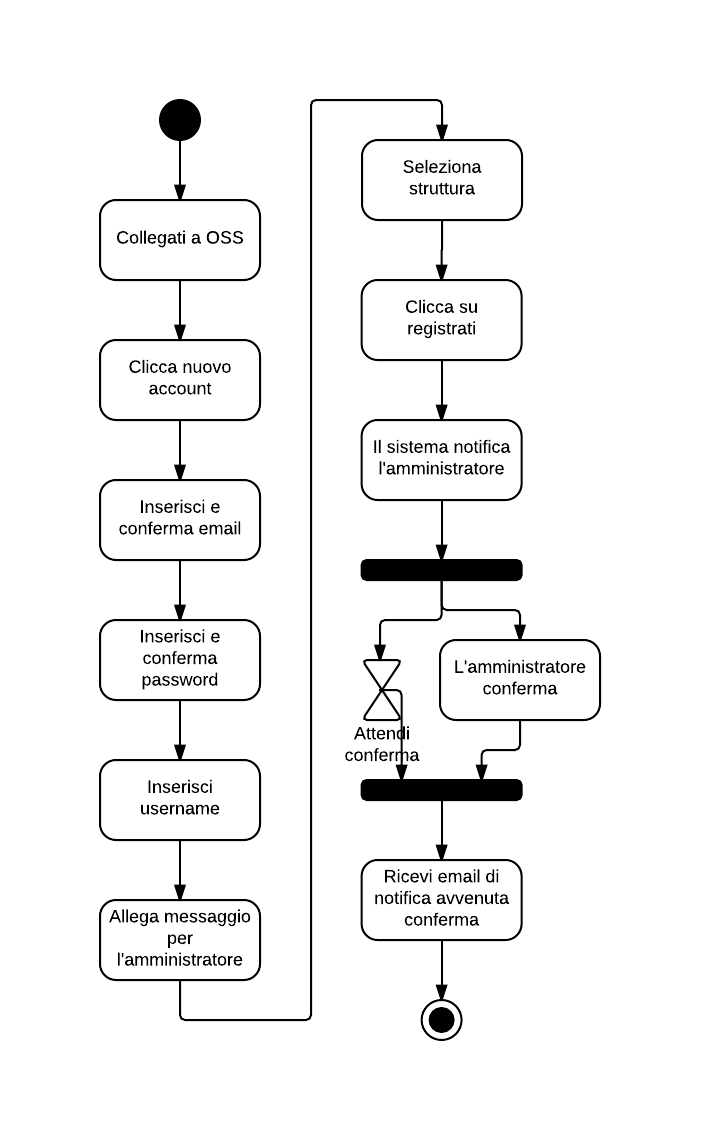
\includegraphics[width=0.6\textwidth]{images/user_new_user.png}
\caption{Diagramma attività: Creazione nuovo account}
\end{figure}


\paragraph{Mokup View}
Di seguito un mockup dell'interfaccia utente per la creazione di un nuovo utente.
I mockup di tutti gli altri casi non vengono creati in quanto banali.
\begin{figure}[H]
\centering
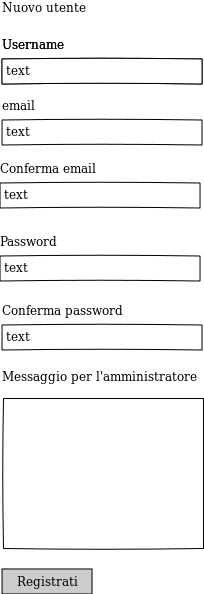
\includegraphics[width=0.3\textwidth]{images/mockup_nuovo_utente.png}
\caption{Mockup nuovo utente}
\end{figure}


\subsubsection{Tdocumentos}\label{tdocumentos}
\def\arraystretch{2}
\begin{table}[H]
\centering
\begin{tabular}{|l|l|}
\hline
Model & Tdocumento \\ \hline
Controller & TdocumentosControllers \\ \hline
View & Tdocumentos \\ \hline
Requisiti & ROU 2, ROU 3, ROU 4, ROU 5, RFU 12, ROO 23, ROO 24, ROS 26 \\ \hline
\end{tabular}
\caption{Tracciamento componente-requisiti Tdocumentos}
\end{table}

\begin{table}[H]
\centering
\begin{tikzpicture}
\node (table) [inner sep=0pt] {
\begin{tabular}{l}
  {TdocumentosController} \\
  \hline
  \\
  \hline
  +index(): void \\
  +view(): void \\
  +add(): void \\
  +edit(): void \\
  +delete(): void \\
  +save(): void \\
  +stampa(): void \\
  +indexbon(): void\\
\end{tabular}
};
\draw [rounded corners=.5em] (table.north west) rectangle (table.south east);
\end{tikzpicture}
\caption{Controller:TdocumentosController}
\end{table}


La vendita di un qualsiasi articolo, PadovaCard compresa, al momento inizia da questo controller, con la creazione di un nuovo documento e l'associazione dell'anagrafica di un cliente. \\

Di seguito viene descritto il processo di vendita della PadovaCard attuale:
\begin{itemize}
\item L'operatore seleziona "Nuovo Documento";
\item L'operatore seleziona un anagrafica cliente, o la crea se non esiste;
\item L'operatore sceglie quale PadovaCard vendere;
\item La vendita si conclude con il pagamento.
\end{itemize}
Mentre con il nuovo sistema il processo di vendità diventerà:
\begin{itemize}
\item Da \tlite viene generato un file di testo, come descritto nella Sezione \ref{progettazionetlite};
\item L'operatore seleziona "Nuovo Documento";
\item L'operatore seleziona un anagrafica cliente, o la crea se non esiste;
\item Il file di testo \tlite corrispondente viene caricato;
\item Il sistema ne estrae i seguenti dati:
	\begin{itemize}
        \item Codice operatore;
        \item Codice cassa;
        \item Codice \tlite;
        \item Elenco di data e ora delle varie visite.
	\end{itemize}
\item L'operatore associa ad ogni visita un pacchetto, un nominativo e una data/ora di inizio validità;
\item Il sistema verifica che tale data comprenda al suo interno la visita alla \cappella;
\item L'operatore visualizza il totale e lo comunica al cliente che decide il metodo di pagamento;
\item Con carta di credito la vendita viene conclusa e il sistema invia all'utente inserito su \tlite una mail contenente i voucher e tutti i dati necessari.
\item Con bonifico bancario il sistema invierà una email all'utente specificando i dati per il versamento, quindi a pagamento effettuato\footnote{Gli operatori controllano quotidianamente gli estratti conto del conto corrente} la carta viene spuntata come attiva.
\end{itemize}

\paragrafo{Diagrammi delle attività}

Di seguito è presentato il diagramma delle attività riguardante il processo di vendita di una PadovaCard. 
\begin{figure}[H]
\centering
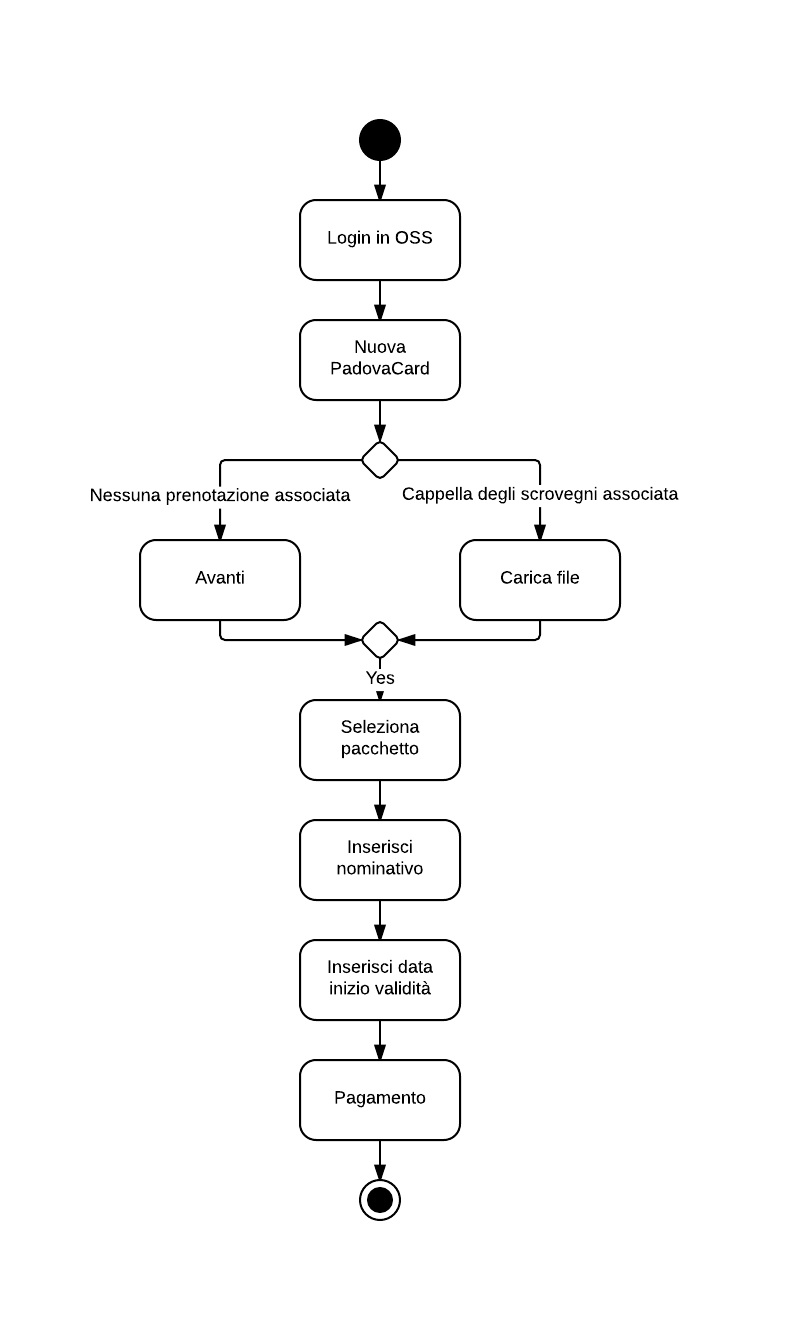
\includegraphics[width=0.6\textwidth]{images/tdocumentos.png}
\caption{Processo di vendita su OSS}
\end{figure}

\paragraph{Caricamento del file testuale}

Vi sono due possibilità, caricamento manuale o automatico.\\
Con il caricamento manuale è l'operatore che dopo aver cliccato su "Nuova Padova Card" dovrà cliccare su "Carica File" quindi selezionare il file corretto.
Il sistema controllerà che la data di creazione del file non sia troppo precedente alla data di apertura (10 minuti). \\

Con il caricamento automatico l'operatore clicca su "Nuova Padova Card" e quindi su "Carica File" ma è OSS che accede alla cratella in cui si trovano i file, carica tutti i files presenti quindi carica i dati del file di proprietà dell'operatore\footnote{All'interno del file c'è sia il codice operatore che il codice cassa, che sarà confrontato con la login di OSS.}. Una volta caricati i dati su OSS il file viene spostato in una cartella diversa che sarà utilizzata come storico.\\ 

In entrambi i casi è possibile non caricare nessun file, se non vi è nessuna prenotazione da associare, cliccando sul tasto "avanti". \\

Si è deciso di utilizzare il caricamento automatico.

\paragraph{Come vengono estratti i dati dal file} 
Per informazioni sul funzionamento del parser vedere la Sezione \ref{parser}.
Il parser ritornerà le informazioni organizzate in un array di questo tipo:
\begin{lstlisting}
array(
	(int) 0 => array(
		'tlite' => 'TLITE0528719557735',
		'data' => '14/05/2015',
		'ora' => '17:15',
		'numero' => '1'
	),
	(int) 1 => array(
		'tlite' => 'TLITE0528719557740',
		'data' => '14/05/2015',
		'ora' => '17:30',
		'numero' => '2'
	)
)
\end{lstlisting}

\paragraph{Funzionamento del pagamento} 
\paragrafo{Contanti} Il pagamento in contanti prevede un'interfaccia con una semplice calcolatrice per il resto.
\paragrafo{Carta di credito} OSS, cosi come altri gestionali sviluppati da \net utilizza una procedura scritta in PHP che si occupa della creazione di una connessione sicura ai circuiti bancari per il pagamento con carta di credito. Tale procedura è separata dal resto del codice, e non verrà modificata. L'interfaccia prevede il form creato da tale procedura e un link per concludere la vendita.
\paragrafo{Bonifico} Oss rende disponibile un link per inviare al cliente una mail con i dati per il bonifico. Dopo aver inviato la mail è possibile concludere il pagamento. \'E compito degli operatori verificare l'estratto conto, al di fuori di OSS per verificare se il cliente ha versato la somma corretta.

\paragraph{Informazioni in possesso dell'utente al termine del processo} 

L'utente la cui anagrafica è stata inserita a livello di documento è l'unico di cui si conosce l'email, pertanto sarà lui il destinatario della mail contenente le informazioni. Tale mail la cui veste grafica è visible nell'Appendice %TODO 
conterrà le seguenti informazioni:
\begin{itemize}
\item Anagrafica del cliente;
\item Numero di PadovaCard acquistate;
\item Totale pagato;
\item I voucher di ogni PadovaCard, ognuno composto da:
	\begin{itemize}
		\item Codice a barre della PadovaCard;
        \item Codice a barre di \tlite (Se presente);
        \item Strutture visitabili con il pacchetto scelto;
        \item Data e ora della visita alla \cappella (Se presente).
	\end{itemize}
\end{itemize}

\paragraph{Informazioni in possesso del sistema al termine del processo}

Il sistema possiede all'interno della cartella utilizzata come storico i file testuali generati da \tlite. \\

All'interno del database è salvato il log delle operazioni nella tabella log, la transazione nella tabella pagamentos e tutti i dati relativi alla PadovaCard nella tabella cards, consultabile alla Sezione \ref{logicorelazionale}.

\paragraph{Possibili errori} 

Nel caso di caricamento del file manuale potrebbe venir caricato il file errato. \\
Nel caso di caricamento automatico del file, se il file non è stato stampato nella cartella condivisa, potrebbe venir caricato un vecchio file. Questo si risolve sia cancellando i file usati dalla cartella condivisa sia controllando l'ora di creazione del file rispetto all'ora corrente, e avvisando l'operatore se queste differsicono troppo. \\
Nel caso in cui le date di attivazione della PadovaCard fossero discordi con le date delle prenotazioni alla \cappella il sistema avverte l'operatore.
Se i nominativi associati alle PadovaCard sono errati l'utente se ne accorgerà quando riceve l'email, in tal caso dovrà chiamare nuovamente e far modificare i nominativi errati.

\paragraph{Acquisto di altri articoli allo IAT} 

Il requisito ROO24 prevede che venga fatto un unico pagamento agli sportelli IAT nel caso in cui l'utente oltre alle PadovaCard acquisti qualcos'altro. Questo è possibile farlo cliccando su "Nuova Riga", visibile sul menu di sinistra nel mockup \ref{perfezionamentoinfo}. Si verrà reindirizzati all'attuale interfaccia di OSS per la vendita.


\paragraph{Mokup View}
Di seguito un mockup del perfezionamento.

\begin{figure}[H] \label{mockupperfezionamento}
\centering
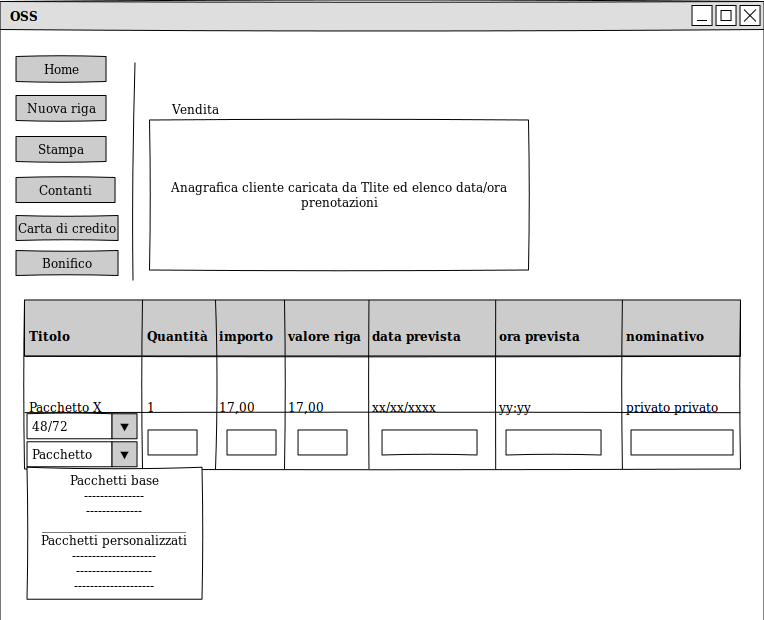
\includegraphics[width=0.8\textwidth]{images/mockup_perfezionamento_info.png}
\caption{Perfezionamento delle informazioni\label{perfezionamentoinfo}}
\end{figure}


\subsubsection{Cards}
\def\arraystretch{2}
\begin{table}[H]
\centering
\begin{tabular}{|l|l|}
\hline
Model & Card \\ \hline
Controller & CardsControllers \\ \hline
View & Card \\ \hline
Requisiti & ROU 6, ROP 17, ROS 28 \\ \hline
\end{tabular}
\caption{Tracciamento componente-requisiti Cards}
\end{table}

\begin{table}[H]
\centering
\begin{tikzpicture}
\node (table) [inner sep=0pt] {
\begin{tabular}{l}
  {CardsController} \\
  \hline
  \\
  \hline
  +index(): void \\
  +view(): void \\
  +search(): void \\
  +edit(): void \\
\end{tabular}
};
\draw [rounded corners=.5em] (table.north west) rectangle (table.south east);
\end{tikzpicture}
\caption{Controller:CardsController}
\end{table}

\paragraph{Validazione PadovaCard}
La view collegata ad index corrisponde a quella in figura \ref{validazionecodicebarre}, e permette all'utente di inserire il codice a barre della PadovaCard, manualmente o tramite il lettore.
Il controller index() prende tale valore e recupera le relative informazioni dal database, per poi mostrarle nella view relativa al metodo view. Le informazioni riportate sono:
\begin{itemize}
\item Nome e cognome del possessore della PadovaCard;
\item Data di inizio e fine validità della PadovaCard;
\item Data e ora della visita alla \cappella se si tratta del relativo personale;
\item Validità dell'ingresso, basandosi sul flag "visitato";
\item Se la visita è già stata effettuata, data e ora di tale visita.
\end{itemize}
Dopo aver recuperato le informazioni dal database imposta il flag visitato ad 1, impedendo un ulteriore visita a tale struttura.\\

Si è voluto rendere il più specifici possibile gli errori che la validazione della PadovaCard ritorna, per permettere al personale delle strutture di precisare il motivo per cui l'utente non può visitare la struttura. I possibili errori sono:
\begin{itemize}
\item \textbf{Struttura già visitata}, l'utente cerca di visitare due volte la stessa struttura;
\item \textbf{PadovaCard non attiva}, la PadovaCard è stata disattivata per un qualche motivo che però non è salvato a sistema;
\item \textbf{Struttura non prevista nel pacchetto}, l'utente si reca in una struttura che non fa parte del pacchetto acquistato;
\item \textbf{Data non valida}, l'utente si reca alla struttura in una data al di fuori del range di validità della PadovaCard;
\item \textbf{PadovaCard non valida}, il codice inserito non appartiene a nessuna PadovaCard presente a sistema;
\item \textbf{Leggere l'altro codice}, il codice inserito non è quello della PadovaCard ma quello \tlite, valido solo per la \cappella.
\end{itemize}

\paragrafo{Diagrammi delle attività}
Di seguito è presentato il diagramma delle attività riguardante il processo di verifica di validità di una PadovaCard da parte del personale delle strutture.

\begin{figure}[H]
\centering
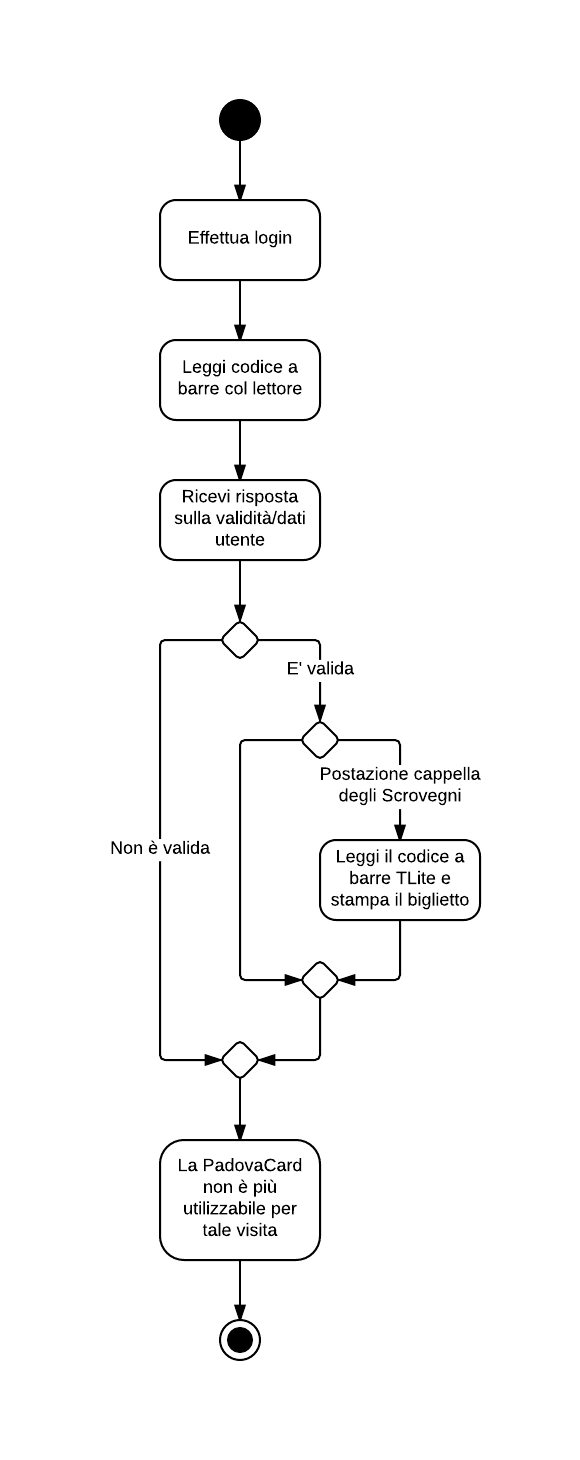
\includegraphics[width=0.6\textwidth]{images/validazione_padovacard.png}
\caption{Processo di verifica della validità della PadovaCard}
\end{figure}


\paragrafo{Mokup View}
Di seguito un mockup delle due viste che ha il personale per validare una PadovaCard. Sarà inserito anche un breve tutorial su come leggere le informazioni riportate sulla PadovaCard e su come utilizzare il lettore di codice a barre. Il risultato della lettura sarà mostrato nella stessa pagina, senza bisogno di refresh.
Notare che il focus per la lettura del codice a barre è già sulla casella di input. \\

Questi accorgimenti mirano a semplificare l'interfaccia il più possibile, e a diminuire il numero di click necessari ad operazione, questo perchè molti degli operatori presenti nelle strutture convenzionate sono anziani volontari o membri di categorie protette, che in entrambi i casi non hanno alcuna famigliarità con il computer.
Con gli adattementi descritti un operatore dovrà solamente inserire nome utente e password quindi scansionare con il lettore le PadovaCard, senza toccare mouse o tastiera.
\begin{figure}[H]
\centering
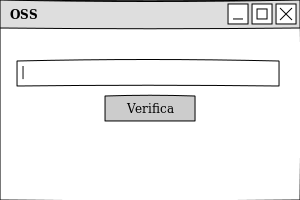
\includegraphics[width=0.5\textwidth]{images/mockup_leggi_barcode.png}
\caption{Schermata per la validazione del codice a barre\label{validazionecodicebarre}}
\end{figure}

\begin{figure}[H]
\centering
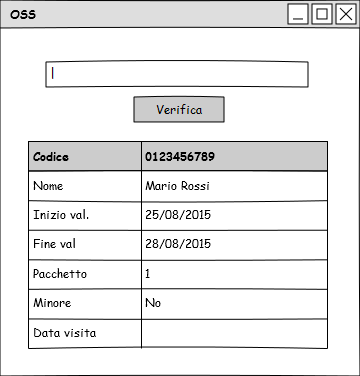
\includegraphics[width=0.5\textwidth]{images/mockup_leggi_barcode2.png}
\caption{Risultato validazione}
\end{figure}


\paragraph{Ricerca/Modifica/Stampa PadovaCard}

Le PadovaCard possono essere ricercate utilizzando il loro codice il nominativo del possessore o quello di chi ha effettuato l'ordine. Una volta recuperata una PadovaCard posso modificarla o visualizzare il dettaglio dell'ordine ia cui appartiene e quindi stamparla. \\

Una volta venduta una PadovaCard si possono compiere solo modifiche che non causano una variazione del suo prezzo. Le modifiche possibili sono dunque:
\begin{itemize}
\item Nominativo del possessore, se la ricerca non è stata fatta col nominativo di chi ha effettuato l'ordine;
\item Data/ora di inizio validità;
\item Codice \tlite solo se già presente, non è quindi possibile aggiungerlo o toglierlo.
\end{itemize}
Per quanto riguarda il codice \tlite, se viene modificato sarà l'operatore a dover andare sul software \tlite, annullare la prenotazione relativa al vecchio codice ed effettuarne una nuova per ottenere il nuovo codice. \\

Nel caso in cui la ricerca sia stata fatta con il nominativo di chi ha fatto l'ordine potrò modificare solo la data/ora di inizio validità, ma non per la singola carta, bensì per tutte le carte. Questo per facilitare un cambio di data nel caso di ordini di molte carte (gruppi, scolaresche etc.). \\

Una PadovaCard può essere stampata solamente agli sportelli IAT, in due occasioni:
\begin{enumerate}
\item L'utente è in possesso del voucher, cartaceo o digitale, ma desidera avere la tessera in cartocnino;
\item L'utente ha smarrito la propria PadovaCard e non è in possesso del voucher, si tratta di un caso meno probabile del precedente.
\end{enumerate}
Nel primo caso all'operatore dello IAT basterà utilizzare il lettore dei codice a barre sul codice del voucher per recuperare i dati, quindi avviare la stampa. \\

Il recupero di una PadovaCard smarrita avviene invece tramite nominativo, per cui l'utente dovrà esibire un documento di riconoscimento all'operatore IAT, il quale recupererà i dati tramite nome e cognome, quindi avvierà la stampa. \\	

La stampa è un semplice bottone che avvia in stampa una PadovaCard sull'apposita stampante.

\paragrafo{Mokup View}
Di seguito un mockup della vista che utilizza l'operatore per la ricerca di una PadovaCard.
\begin{figure}[H]
\centering
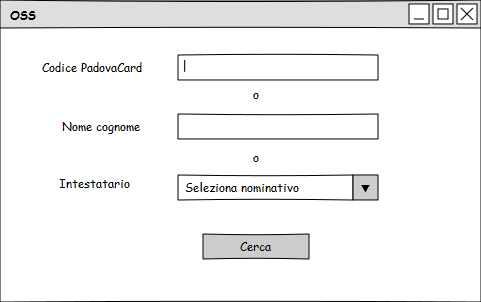
\includegraphics[width=0.7\textwidth]{images/mockup_stampa_tessera.png}
\caption{Schermata per la ricerca di una PadovaCard\label{stampaPadovaCard}}
\end{figure}

Nell'immagine seguente si vede un mockup della vista per la visualizzazione dei risultati, nella parte superiore può apparire un elenco di PadovaCard tra cui scegliere nel caso in cui la ricerca venga fatta tramite nominativo, e siano presenti più carte appartenenti allo stesso nominativo. Nel caso in cui la ricerca venga fatta tramite intestatario e tale persona ha più ordini salvati nel sistema, si potrà scegliere quale ordine modificare.

\begin{figure}[H]
\centering
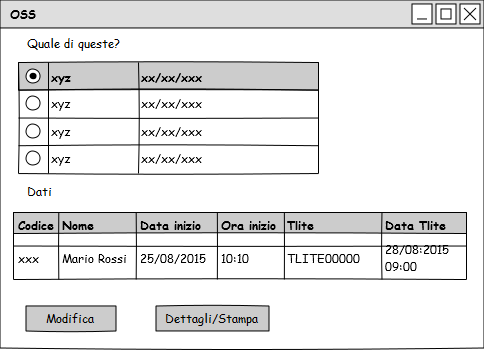
\includegraphics[width=0.7\textwidth]{images/mockup_dettagli_ricerca.png}
\caption{Schermata per visualizzare i dettagli di una ricerca}
\end{figure}

\paragrafo{Diagrammi delle attività}
Di seguito è presentato il diagramma delle attività riguardante il processo di modifica della data di validità e del nominativo associati ad una PadovaCard.
\begin{figure}[H]
\centering
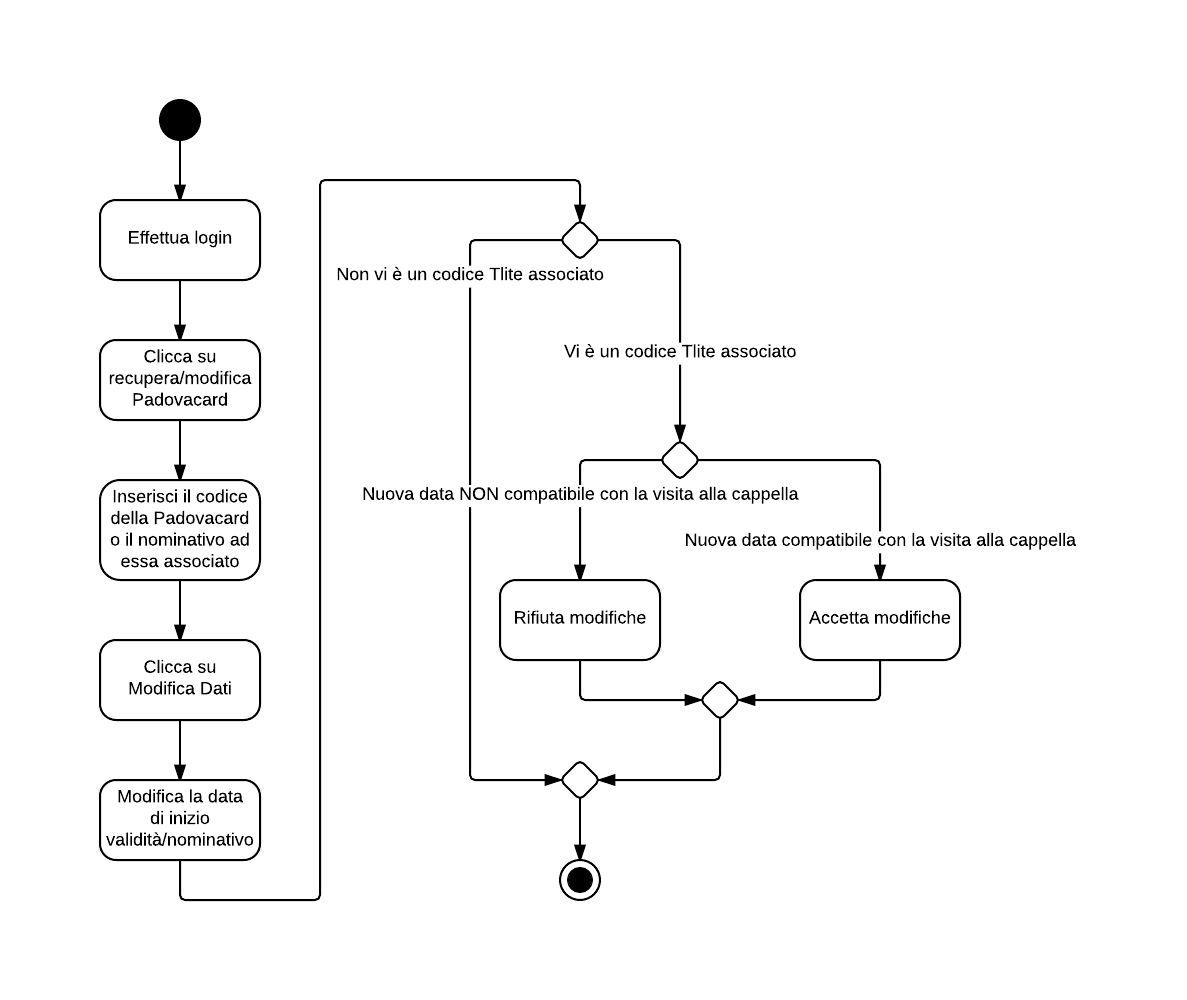
\includegraphics[width=1\textwidth]{images/modifica_padovacard.png}
\caption{Processo di modifica dati PadovaCard}
\end{figure}

\subsubsection{Gestione bonifici}
Acquistando tramite call center è possibile effettuare il pagamento via bonifico.
La procedura d'acquisto della PadovaCard rimane uguale a quanto descritto nella Sezione \ref{tdocumentos} e quando si seleziona pagamento tramite bonifico il cliente riceve un email dove vengono specificati conto corrente, causale e importo da versare. Il cliente ha due giorni per effettuare il bonifico e confermare il versamento via email. Gli operatori controlleranno quindi l'estratto conto e in caso positivo concluderanno la vendita e il cliente riceverà i voucher. \\

Oltre all'email con i dati per il pagamento è necessario realizzare un interfaccia che permetta agli operatori di vedere i pagamenti in sospeso e di concluderli. L'index di Tdocumentos mostra già i propri ordini, sia chiusi che pendenti, ma in questo caso ogni operatore ha la necessità di vedere gli ordini di tutti gli operatori in quanto chi effettua l'ordine non è necessariamente colui che lo conclude. Per questo si è deciso di creare una nuova vista dove sono elencati solo i pagamenti via bonifico in attesa di conferma. Per confermare un pagamento si entrerà tramite link alla view dei dettagli dell'ordine. Gli ordini scaduti verranno eliminati.

\paragrafo{Mokup View}
Nell'immagine seguente si vede un mockup della schermata che visualizza i risultati ritornati da una ricerca.

\begin{figure}[H]
\centering
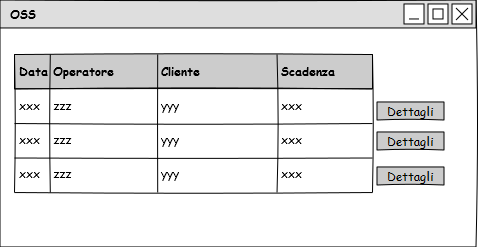
\includegraphics[width=0.7\textwidth]{images/mockup_vista_bonifico.png}
\caption{Schermata per visualizzare i dettagli di una ricerca}
\end{figure}


\subsection{Tracciamento requisiti}\label{tracciamento}

\begin{center}
\def\arraystretch{2}
\begin{longtable}{|p{7cm}|p{3cm}|}
\cellcolor[gray]{0.9} \textbf{Componente} & \cellcolor[gray]{0.9} \textbf{Requisiti} \\ \hline
Users & ROP 14 \newline ROP 15 \newline ROP 16 \newline RFP 18 \newline ROO 19 \newline ROO 20 \newline ROO 21 \\ \hline
Tdocumentos & ROU 2 \newline ROU 3 \newline ROU 4 \newline ROU 5 \newline RFU 12 \newline ROO 23 \newline ROO 24 \newline ROS 26 \\ \hline
Cards & ROU 6 \newline ROP 17 \newline ROS 28 \\ \hline
Cards & ROU 7 \\ \hline
Cards & ROO 25 \newline RFO 31 \\ \hline
\caption{Tracciamento componenti - requisiti}
\end{longtable}

\def\arraystretch{2}
\begin{longtable}{|p{7cm}|p{3cm}|}
\cellcolor[gray]{0.9} \textbf{Requisito} & \cellcolor[gray]{0.9} \textbf{Componenti} \\ \hline
ROU 1 & \\ \hline
ROU 2 & Tdocumentos \\ \hline
ROU 3 & Tdocumentos \\ \hline
ROU 4 & Tdocumentos \\ \hline
ROU 5 & Tdocumentos \\ \hline
ROU 6 & Cards \\ \hline
ROU 7 & Cards \\ \hline
RFU 8 & \\ \hline
RFU 9 & \\ \hline
RFU 10 & \\ \hline
RFU 11 & \\ \hline
RFU 13 & \\ \hline
ROP 14 & User \\ \hline
ROP 15 & User \\ \hline
ROP 16 & User \\ \hline
ROP 17 & Cards \\ \hline
RFP 18 & User \\ \hline
ROO 19 & User \\ \hline
ROO 20 & User \\ \hline
ROO 21 & User \\ \hline
ROO 22 & \tlite \\ \hline
ROO 23 & Tdocumentos \\ \hline
ROO 24 & Tdocumentos \\ \hline
ROO 25 & Cards \\ \hline
ROS 26 & Tdocumentos \\ \hline
ROS 27 & \\ \hline
ROS 28 & Cards \\ \hline
ROS 29 & \\ \hline
RFS 30 & \\ \hline
RFO 31 & Cards \\ \hline
\caption{Tracciamento requisiti - componenti}
\end{longtable}

\end{center} 


\subsection{Tracciamento requisiti}\label{tracciamento}


\begin{center}
\def\arraystretch{2}
\begin{longtable}{|p{7cm}|p{3cm}|}
\cellcolor[gray]{0.9} \textbf{Componente} & \cellcolor[gray]{0.9} \textbf{Requisiti} \\ \hline
Users & ROP 14 \newline ROP 15 \newline ROP 16 \newline RFP 18 \newline ROO 19 \newline ROO 20 \newline ROO 21 \\ \hline
Tdocumentos & ROU 2 \newline ROU 3 \newline ROU 4 \newline ROU 5 \newline RFU 12 \newline ROO 23 \newline ROO 24 \newline ROS 26 \\ \hline
Visits & ROU 6 \newline ROP 17 \newline ROS 28 \\ \hline
Prints & ROU 7 \\ \hline
EditPadovaCard & ROO 25 \newline RFO 31 \\ \hline
\caption{Tracciamento componenti - requisiti}
\end{longtable}

\def\arraystretch{2}
\begin{longtable}{|p{7cm}|p{3cm}|}
\cellcolor[gray]{0.9} \textbf{Requisito} & \cellcolor[gray]{0.9} \textbf{Componenti} \\ \hline
1 & \\ \hline
ROU 2 & Tdocumentos \\ \hline
ROU 3 & Tdocumentos \\ \hline
ROU 4 & Tdocumentos \\ \hline
ROU 5 & Tdocumentos \\ \hline
ROU 6 & Visits \\ \hline
ROU 7 & Prints \\ \hline
RFU 8 & \\ \hline
RFU 9 & \\ \hline
RFU 10 & \\ \hline
RFU 11 & \\ \hline
RFU 12 & Tdocumentos \\ \hline
RFU 13 & \\ \hline
ROP 14 & User \\ \hline
ROP 15 & User \\ \hline
ROP 16 & User \\ \hline
ROP 17 & Visits \\ \hline
RFP 18 & User \\ \hline
ROO 19 & User \\ \hline
ROO 20 & User \\ \hline
ROO 21 & User \\ \hline
ROO 22 & \tlite \\ \hline
ROO 23 & Tdocumentos \\ \hline
ROO 24 & Tdocumentos \\ \hline
ROO 25 & EditPadovaCard \\ \hline
ROS 26 & Tdocumentos \\ \hline
27 & \\ \hline
ROS 28 & Visits \\ \hline
29 & \\ \hline
30 & \\ \hline
31 & EditPadovaCard \\ \hline
\caption{Tracciamento requisiti - componenti}
\end{longtable}

\end{center} 
% DI TUTTO UN PO'

\subsection{Veste grafica PadovaCard}null


Utilzzo di https
\appendix
\addappheadtotoc
\setcounter{table}{0}
\renewcommand{\thetable}{A.\arabic{table}}
%\clearpage\null\newpage
\pagebreak
\section{Verbale del  27/01/2015}\label{verbale}
\begin{itemize}
\item \textbf{Luogo:} Sede di Ne-t by Telerete Nordest s.r.l, Via Salboro 22/b - 35124 Padova (PD);
\item \textbf{Data:} 27/01/2015;
\item \textbf{Ora:} 11:00;
\item \textbf{Durata:} 2 ore;
\item \textbf{Partecipanti interni:} Carlo Bettin, Giuliano Fiocco, Gino Marconato, Andrea Rampado, Nicolò Tresoldi;
\item \textbf{Partecipanti esterni:} Team di Charta.

\end{itemize}
Durante la riunione sono state prese le seguenti decisioni:
\begin{itemize}
\item La modalità di acquisto via web viene spostata da requisito obbligatorio a requisito opzionale e verrà quindi implementata in un secondo momento, la progettazione del sistema deve comunque tenerne conto per evitare che la futura implementazione richieda costi troppo elevati;
\item L'acquisto via hotel non permetterà più la personalizzazione dei pacchetti, si tratterà quindi di un semplice accesso preferenziale al call center;
\item Sia la vendita allo IAT che la vendita tramite call center prevede l'acquisto di un biglietto d'ingresso alla cappella degli Scrovegni a costo zero, acquistato dal cliente Telerete. Tale acquisto è direttamente confermato e non prevede una successiva conferma manuale da parte dell'operatore;
\item L'operatore effettuato l'acquisto copierà il codice Tlite sul sistema OSS e inserirà qui l'anagrafica del cliente, il tipo di pacchetto e l'inizio del periodo di validità;
\item Il cliente effettuerà il pagamento sulla piattaforma OSS, e nel caso l'operazione non andasse a buon fine l'operatore deve tornare su Tlite e annullare la prenotazione;
\item Allo IAT è inoltre possibile personalizzare il pacchetto dopo la prenotazione su Tlite e prima del pagamento.
\end{itemize}

Per raggiungere tali obbiettivi \charta dovrà fornire le seguenti funzionalità:
\begin{itemize}
\item Inserire un biglietto a zero euro per la \cappella;
\item Eliminare le attuali PadovaCard;
\end{itemize}



%\section{Glossario}
\definizione{CakePhp}: framework per la realizzazione di applicazioni web scritto in PHP. È ispirato al concetto di \glossario{MVC}. \\
\definizione{IAT} Acronimo di Informazioni assistenza turistica, si tratta degli uffici o sportelli sparsi per la città in cui si possono ottenere informazioni, e acquistare/ricevere la PadovaCard. \\
\definizione{MVC}: Acronimo di Model View Controller, è un Design Pattern architetturale che divide l’applicazione in tre parti interconnesse, separando l’interfaccia utente, la logica e i dati. \\
\definizione{Operatore}: si tratta di operatori degli sportelli \glossario{IAT} o del call center;\\
\definizione{OSS}:  \\
\definizione{Personale}: si tratta del personale delle \glossario{strutture} convenzionate con PadovaCard, si occuperanno di verificarne la validità. \\
\definizione{Struttura}: si fa riferimento alle strutture convenzionate con PadovaCard, e quindi visitabili dagli \glossario{utenti} che ne sono in possesso \\
\definizione{Utente}: si tratta del fruitore della PadovaCard, tipicamente un turista.\\
\definizione{Voucher}: documenti emessi da agenzie di viaggio ai propri clienti, come conferma del diritto a godere, nel loro viaggio, di specifici servizi, in essi indicati e già pagati in precedenza all'agenzia stessa. In questo caso si tratta di un foglio formato A4 stampato dall'hotel che ha il valore di una PadovaCard in quanto su di esso è riportato il codice a barre relativo. \\
  

\end{document}